\documentclass[]{article}
\usepackage[UTF8]{ctex}
\usepackage[top=2.5cm, bottom=2cm, left=2.5cm, right=2.5cm]{geometry}
\usepackage{url}
\usepackage{graphicx}
\usepackage{float}
\usepackage{cite}
\usepackage{fancyhdr}
\usepackage{multicol}

\pagestyle{fancy}
\setlength{\parindent}{2pt} % 设置开头的缩进
% 更改摘要和关键词标题为英文
\renewcommand{\abstractname}{Abstract}
% 添加关键词命令
\newcommand{\keywords}[1]{\textbf{Keywords:} #1}
%opening
\title{Raft 一致性协议的实现}
\author{刘芳新\\ \footnotesize 中山大学~~智能科学与技术~~21312482}
\date{2023 年 12 月 16 日} % 取消自动显示日期
\begin{document}
	% \twocolumn[
	\maketitle
	\thispagestyle{fancy} % 仅在标题页使用自定义的页眉设置
	%\begin{abstract}
		%\hspace{1em}本课程设计报告探讨了Kaggle举办的FGVC8(CVPR2021-workshop)Plant Pathology-2021数据集分类任务。通过将标签进行独热编码转化为多标签分类问题,我们研究了两种卷积神经网络模型来解决本分类任务。本报告分析了Plant Pathology-2021数据集的样本细节,并详细介绍了LeNet模型与Vision Transformer模型的构建、训练与优化过程以及它们在Plant Pathology-2021分类任务上不同的性能差距。我们还讨论了ArcFaceLoss与CrossEntropyLoss在本任务上的效果对比,以及对比数据集裁剪的效果。最后,本报告提出了一些可能的优化方向。
	%\end{abstract}
	
	% \keywords{one-hot,LeNet,VIT,Plant Pathology-2021,ArcFaceLoss}
	\vfill
	\hrule
	\footnotesize
	\vspace{12pt} % 插入12点的垂直空间
	\begin{minipage}{\textwidth}
		\raggedright % 左对齐
		学号: 21312482 \\ 
		课程: 分布式计算实验 \\ 
		日期:2023年12月16日 \\ 
		Email:liufx7@mail2.sysu.edu.cn
	\end{minipage}
	\normalsize 
	\newpage % 分页命令
	\tableofcontents % 生成目录页
	\newpage % 分页命令
	\section{lab2-A leader election}
	\subsection{任务分析}
	Raft算法是一种分布式一致性算法,设计用于确保在分布式系统中的多个节点之间达成一致性。Raft将整个系统的状态分为任期(term)、领导者(leader)和跟随者(follower)三个状态,并通过领导者选举机制和心跳机制来维持整个系统的一致性。

	在Raft中,系统中的节点通过领导者选举机制来选出一个领导者。节点首先以跟随者的身份启动,在一段时间内未收到领导者的心跳时,它们会发起一次选举。选举的过程中,节点会向其他节点发送投票请求,其他节点通过比较各自的任期和候选节点的任期来决定是否投票。如果候选节点获得多数票,它将成为新的领导者。

	Raft中的领导者通过定期向其他节点发送心跳来维持其领导地位。这些心跳包告诉其他节点当前的领导者仍然处于活跃状态。如果一个节点在一定时间内没有收到来自领导者的心跳,它就会启动新的选举过程,试图成为新的领导者。

	在Lab 2A中,我们需要实现Raft领导者选举和心跳机制的一部分。具体来说涉及到以下几个方面:
	\begin{itemize}
	\item 实现节点状态的切换:节点在不同的状态(跟随者、候选者、领导者)之间切换,具体取决于收到的消息和定时器的触发。
	\item 实现选举过程:包括候选者的发起、投票的请求和回复等。
	\item 实现心跳机制:领导者定期向其他节点发送心跳消息。
	\end{itemize}

	\subsection{功能设计}
	\subsubsection{完善Raft结构体}
	在raft结构体内,我添加了paper中Figure2中提及到的变量。
	\begin{figure}[H]
		\centering
		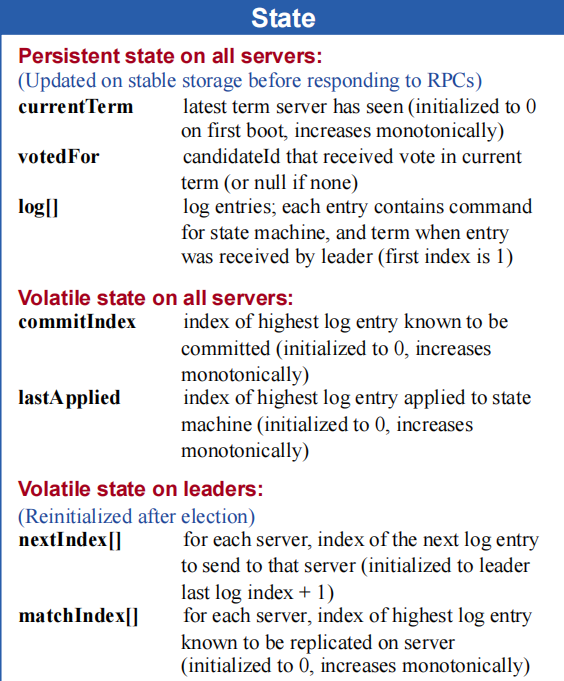
\includegraphics[width=0.4\textwidth]{./figure1.png}
		\caption{paper中figure2关于Raft结构体的部分}
	\end{figure}
	
	除此之外,我还添加了以下变量:
	\begin{itemize}
	\item state:节点状态(leader/follower/candidate)
	\item lastLogIndex:最后一个日志条目的索引
	\item lastLogTerm:最后一个日志条目的任期
	\item ElectionStatus:这个变量用于表示发生了什么事件。
	
	=0:这个变量的初始化
	
	=1:follower阶段的计时器超时,应当转变为candidate发起election
	
	=2:candidate收集到了足够的票数,应当转变为leader
	
	=3:candidae在投票选举过程中超时了,应当更新term,发起新的一轮election
	
	= -1:表示raft实例接受到了消息,需要重置timer,并且自己的身份已经转变为了follower。例如:收到来自leader的ae消息、投票给了其他raft实例等。
	
	\item mesMutex:这是一个互斥锁,由于raft结构体中的变量诸多,这么多变量都只用一个锁的话,我觉得会导致go routine之间的性能降低,因此添加了这个互斥锁用于访问ElectionStatus这个使用频率很高的变量。
	
	\item messageCond:这是一个条件变量,以mesMutex作为它的互斥锁。一个raft实例在等待ElectionStatus的变化来决定后续的操作的时候,可以通过wait这个条件变量,当ElectionStatus发生改变的时候,就需要对messageCond进行广播,对等待ElectionStatus的go routine即可被唤醒继续执行。举例来说:一个follower在开始阶段,ElectionStatus=0,需要等待后续事件,如果发生timeout,则ElectionStatus=1;如果收到投票要求并成功投票,则ElectionStatus=-1,后续需要重置timer等。
	
	\item changeElectionStatus函数:由于mesMutex这是一个针对ElectionStatus变量的互斥锁,每次修改这个变量都需要对这个锁操作,因此将修改操作封装到了一个函数中。
	\end{itemize}
	\par
	注意:在同时查看ElectionStatus变量和调用changeElectionStatus函数时存在潜在的死锁风险。这是因为在查看ElectionStatus变量之前需要获取锁,如果在没有释放锁的情况下直接调用changeElectionStatus,由于changeElectionStatus函数也需要获取锁,可能会导致无法获得所需的锁,从而产生死锁。
	\subsubsection{完善GetState函数}
	GetState 返回当前节点的任期和该节点是否认为自己是领导者
	\subsubsection{完善RequestVote功能}
	先按照paper中的figure2实现RequestVoteArgs和RequestVoteReply结构体。
	\begin{figure}[H]
		\centering
		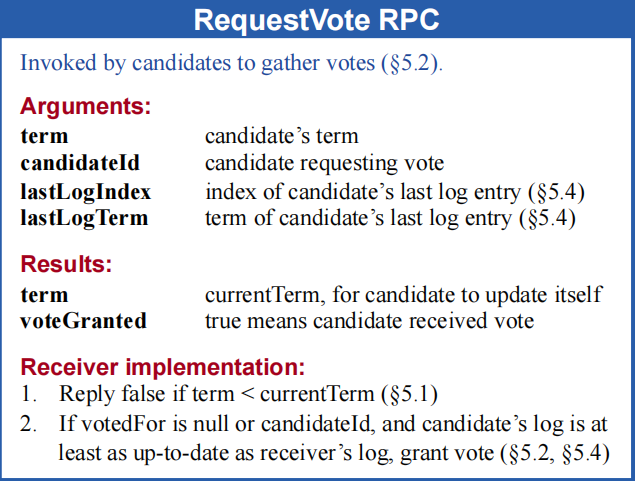
\includegraphics[width=0.4\textwidth]{./figure2.png}
		\caption{paper中figure2关于RequestVote的部分}
	\end{figure}
	然后按照以下规则完善RequestVote函数:
	\begin{itemize}
		\item 如果请求的任期小于当前任期,则拒绝投票
		\item 如果请求的最后一个日志条目的任期小于节点的最后一个日志条目的任期,则拒绝投票
		\item 如果节点已经投过票给其他节点,则拒绝投票
		\item 如果请求的任期大于当前任期,则更新当前任期,同意投票,并转变为 follower 状态
	\end{itemize}
	\subsubsection{实现AppendEntries功能}
	Leader会周期性地给其他节点发送ae消息,这个RPC调用首先需要实现参数和返回值的结构体设计,结构体的设计直接参照paper即可。同时仿照sendRequestVote写了sendAppendEntries函数。
	\begin{figure}[H]
		\centering
		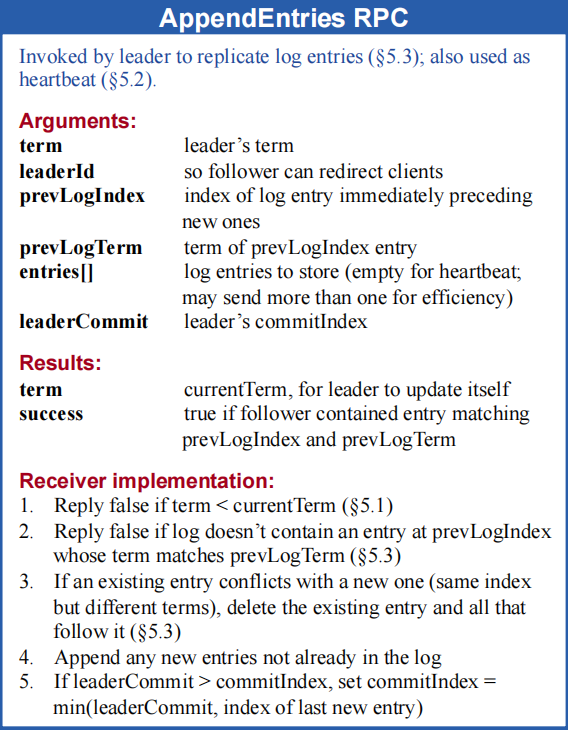
\includegraphics[width=0.4\textwidth]{./figure3.png}
		\caption{paper中figure2关于AppendEntries的部分}
	\end{figure}
	设计AppendEntries函数,当节点收到AE消息后,执行以下步骤:
	
	1.检查Leader的Term是否更大。如果Leader的Term不大于当前节点的Term,则直接返回false并携带当前节点的Term。如果Leader的Term较大,则进行下一步骤。
	
	2.认可新的Leader,并将节点的Term和Leader的Term保持一致。节点将自身状态重置为Follower的初始状态,重新启动选举计时器。随后,通过messageCond.Broadcast()通知节点及时处理后续消息。
	
	\subsubsection{完善ticker函数}
	在 ticker() 函数中,该函数是大多数节点一直在运行的。以下是该函数的任务流程:
	\begin{enumerate}
	\item 作为Follower,初始化ElectionStatus为0,并设置计时器以检测超时。如果收到AppendEntries或者投票给了其他节点,ElectionStatus将被设定为-1。如果计时器时间到了,发现ElectionStatus不等于-1,说明在这段时间内,节点没有收到AppendEntries或者投票,那么就是发生了超时,将ElectionStatus设定为1。否则,节点在这段时间内发生了某些活动,已经重新发起了一个新的计时器,这个计时器没有实际意义,因此无需将ElectionStatus设定为1。
	
	\item 如果发现ElectionStatus为1,则将状态转变为Candidate,并向其他节点发起RequestVote RPC调用,然后进入步骤3。
	
	\item 如果发现ElectionStatus为-1,返回到初始步骤1。
	
	\item 在投票阶段,再次启动一个计时器。如果计时器时间到了,发现ElectionStatus不等于-1,说明发生了超时,将ElectionStatus设定为3,表示投票阶段超时。
	
	\item 在投票阶段,ticker()函数再启动两个新的协程:一个用于处理投票的协程vThread,另一个用于投票阶段的计时器协程tThread。然后进入阻塞状态,等待消息。
	
	负责投票的协程vThread:通过创建新的协程向其他Raft节点发起投票RPC调用,并创建一个条件变量voteCond。voteCond.Wait()用于等待每个投票RPC调用的成功,并在成功后通过voteCond.Broadcast唤醒vThread。
	
	投票阶段计时器协程tThread:类似于初始阶段的计时器,设置一个随机时间。如果到时了,尝试将ElectionStatus设置为3。如果ElectionStatus为-1或4,表示节点已经不是Candidate,投票阶段已经结束,直接退出。否则,将ElectionStatus设置为3,并通知ticker()协程重新启动一次投票。
	
	\item ticker()被唤醒后,根据ElectionStatus的不同值进行不同的处理:
	
	如果ElectionStatus为2,表示节点已经是Leader。此时,启动一个新的协程周期性地发送心跳,然后阻塞本协程直到节点不再是Leader。然后返回到初始状态的步骤1。
	
	如果ElectionStatus为3,表示投票阶段超时,需要重新发起新的投票。
	
	如果ElectionStatus为4或-1,表示节点不再是Candidate,需要回到初始状态的步骤1。
	\end{enumerate}
	\subsubsection{实现heartbeat函数}
	heartBeats函数由Leader调用,用于周期性向其他Raft节点发送AppendEntries消息。
	
	根据实验规定,心跳的周期不得超过每秒10次。因此,我设置了每秒10次的频率,同样通过使用time.Sleep来实现。
	
	由于Lab2A仅需要实现选举功能,无需考虑日志的事务。因此,该函数的逻辑非常简单。在每个周期内,向其他的Raft节点发送AppendEntries消息。注意,这个发送AppendEntries消息是一个RPC调用,因此应当新开一个协程来进行发送,以避免阻塞heartBeats协程。
	
	如果在发送AppendEntries消息后,收到的返回消息中发现有某个Raft节点的Term值比自身还高,说明自身已经过时。此时,将自己变为Follower,并更新自身的Term值,同时将voteFor初始化为-1。
	
	\subsubsection{完善Make函数}
	Make函数就是完成raft节点的初始化即可。
	
	\subsection{代码实现}
	\begin{itemize}
		\item 完善Raft结构体
		\begin{figure}[H]
			\centering
			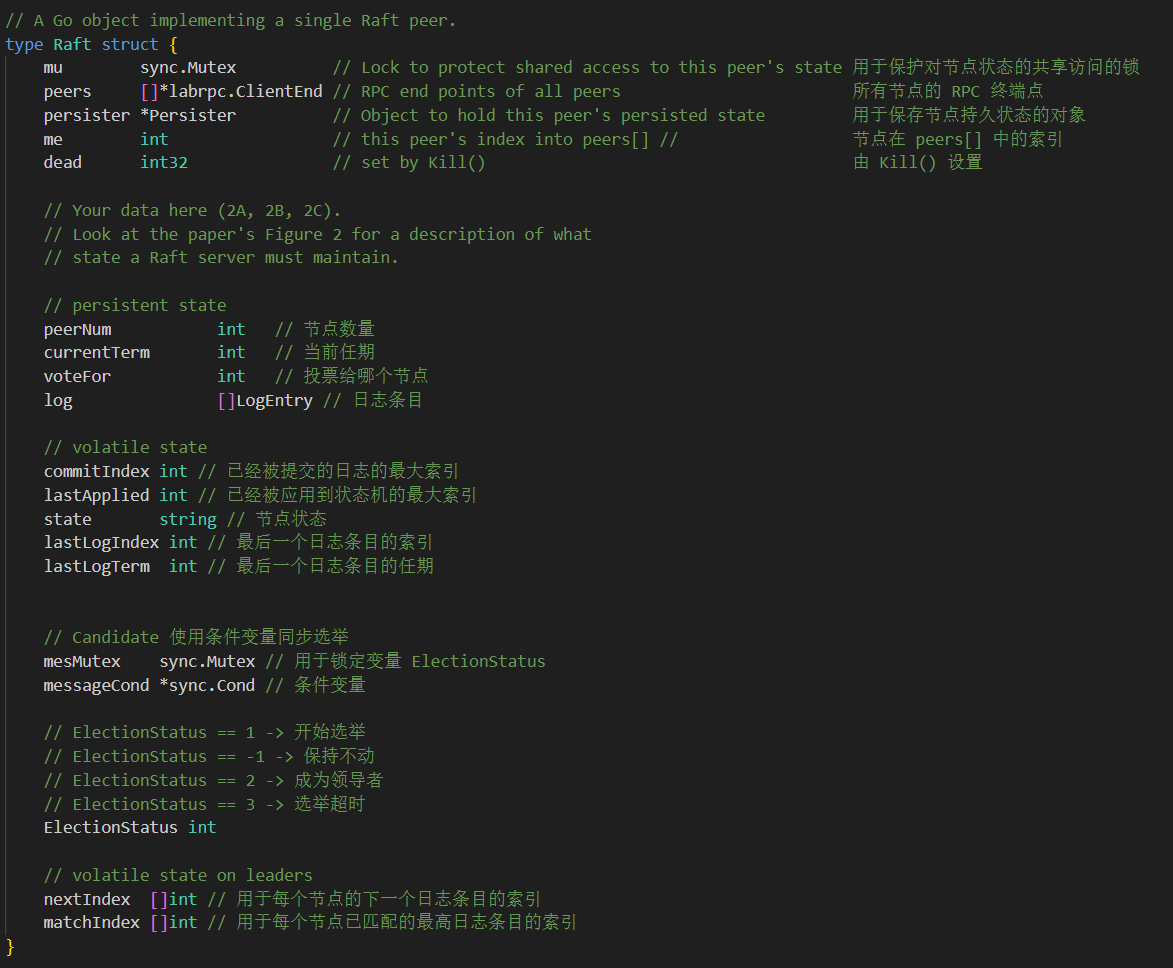
\includegraphics[width=0.8\textwidth]{./2A/Raft.png}
			\caption{Raft结构体}
		\end{figure}
		\begin{figure}[H]
			\centering
			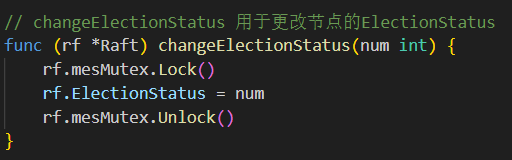
\includegraphics[width=0.8\textwidth]{./2A/changeElectionStatus.png}
			\caption{changeElectionStatus函数}
		\end{figure}
		\item 完善GetState函数
		\begin{figure}[H]
			\centering
			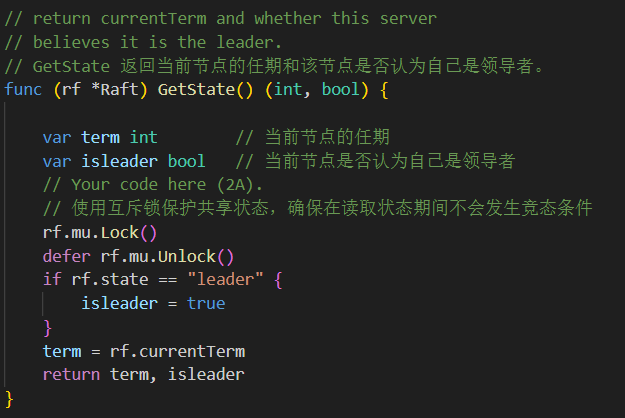
\includegraphics[width=0.8\textwidth]{./2A/GetState.png}
			\caption{GstState函数}
		\end{figure}
		\item 完善Request Vote功能
		\begin{figure}[H]
			\centering
			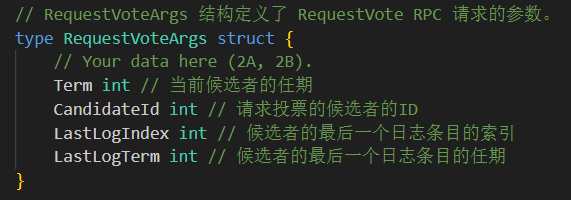
\includegraphics[width=0.8\textwidth]{./2A/RequestVoteArgs.png}
			\caption{RequestVoteArgs结构体}
		\end{figure}
		\begin{figure}[H]
			\centering
			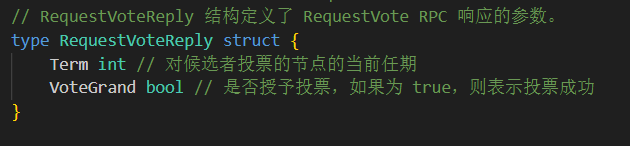
\includegraphics[width=0.8\textwidth]{./2A/RequestVoteReply.png}
			\caption{RequestVoteReply结构体}
		\end{figure}
		\begin{figure}[H]
			\centering
			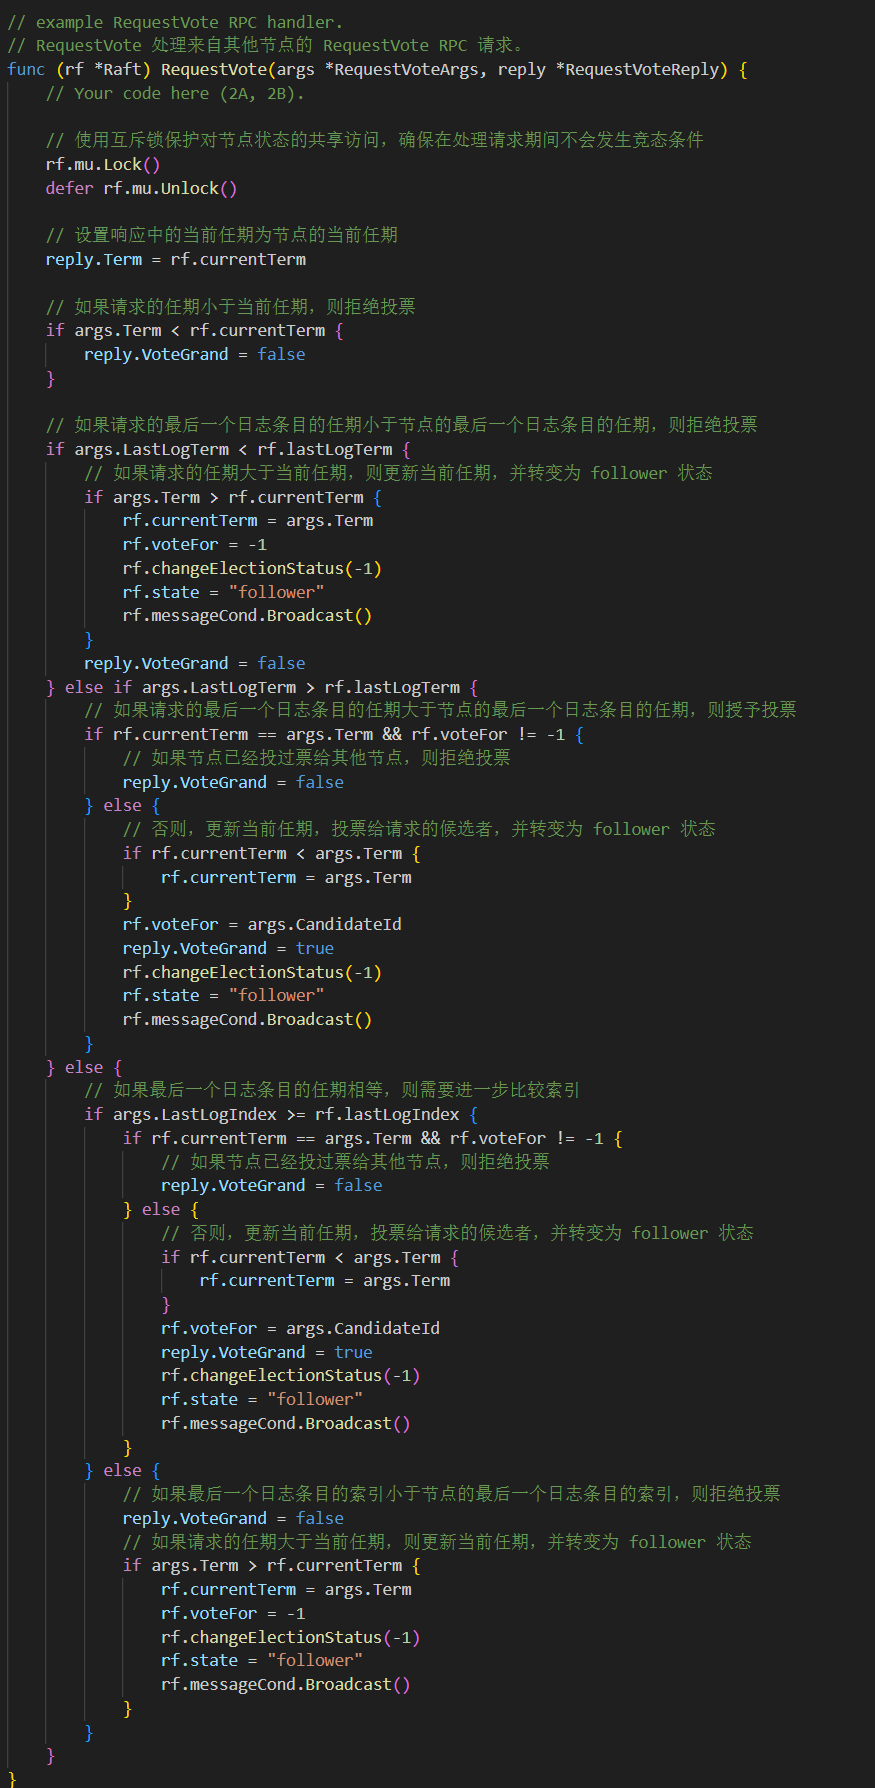
\includegraphics[height=0.95\textheight]{./2A/RequestVote.png}
			\caption{RequestVote函数}
		\end{figure}
		\item 实现AppendEntries功能
		\begin{figure}[H]
			\centering
			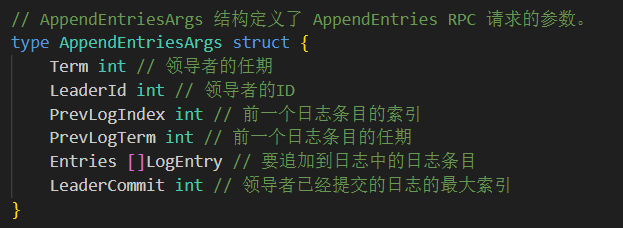
\includegraphics[width=0.8\textwidth]{./2A/AppendEntriesArgs.png}
			\caption{AppendEntriesArgs结构体}
		\end{figure}
		\begin{figure}[H]
			\centering
			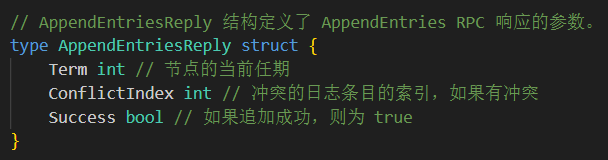
\includegraphics[width=0.8\textwidth]{./2A/AppendEntriesReply.png}
			\caption{AppendEntriesReply结构体}
		\end{figure}
		\begin{figure}[H]
			\centering
			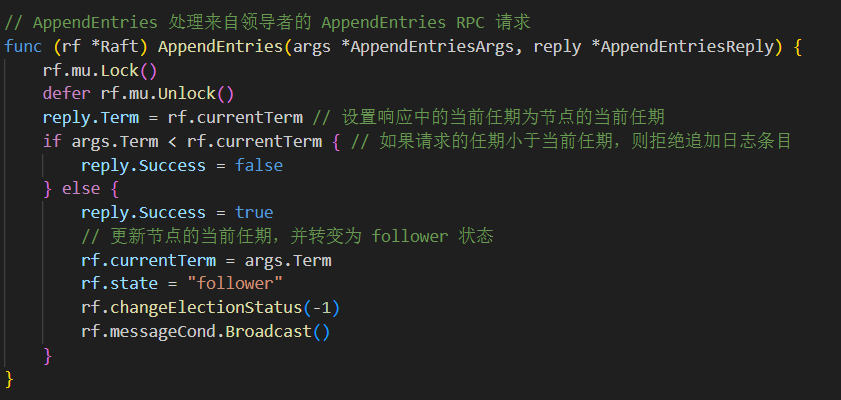
\includegraphics[width=0.8\textwidth]{./2A/AppendEntries.png}
			\caption{AppendEntries函数}
		\end{figure}
		\item 完善ticker函数
		\begin{figure}[H]
			\centering
			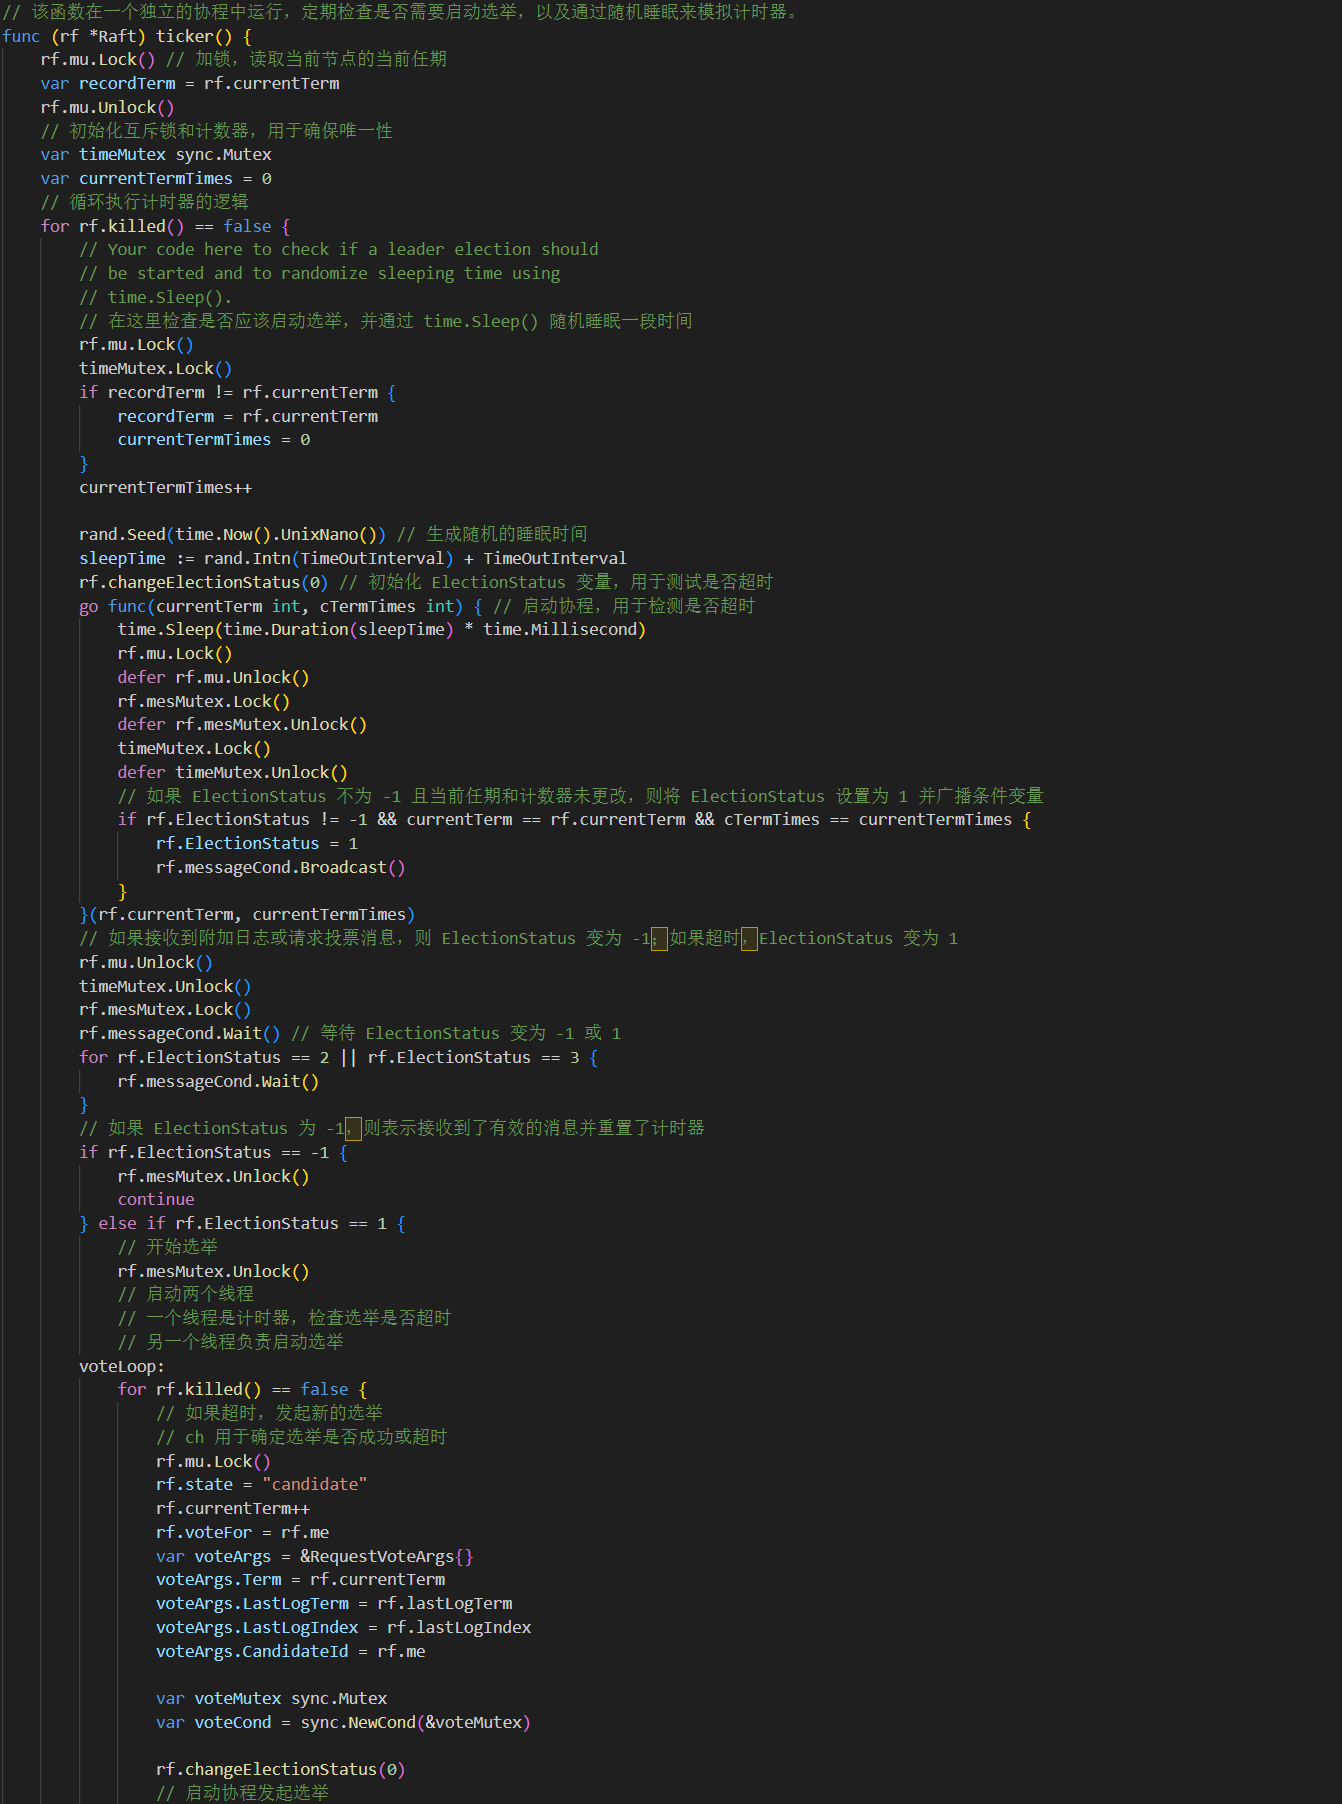
\includegraphics[height=1\textheight]{./2A/ticker1.png}
		\end{figure}
		\begin{figure}[H]
			\centering
			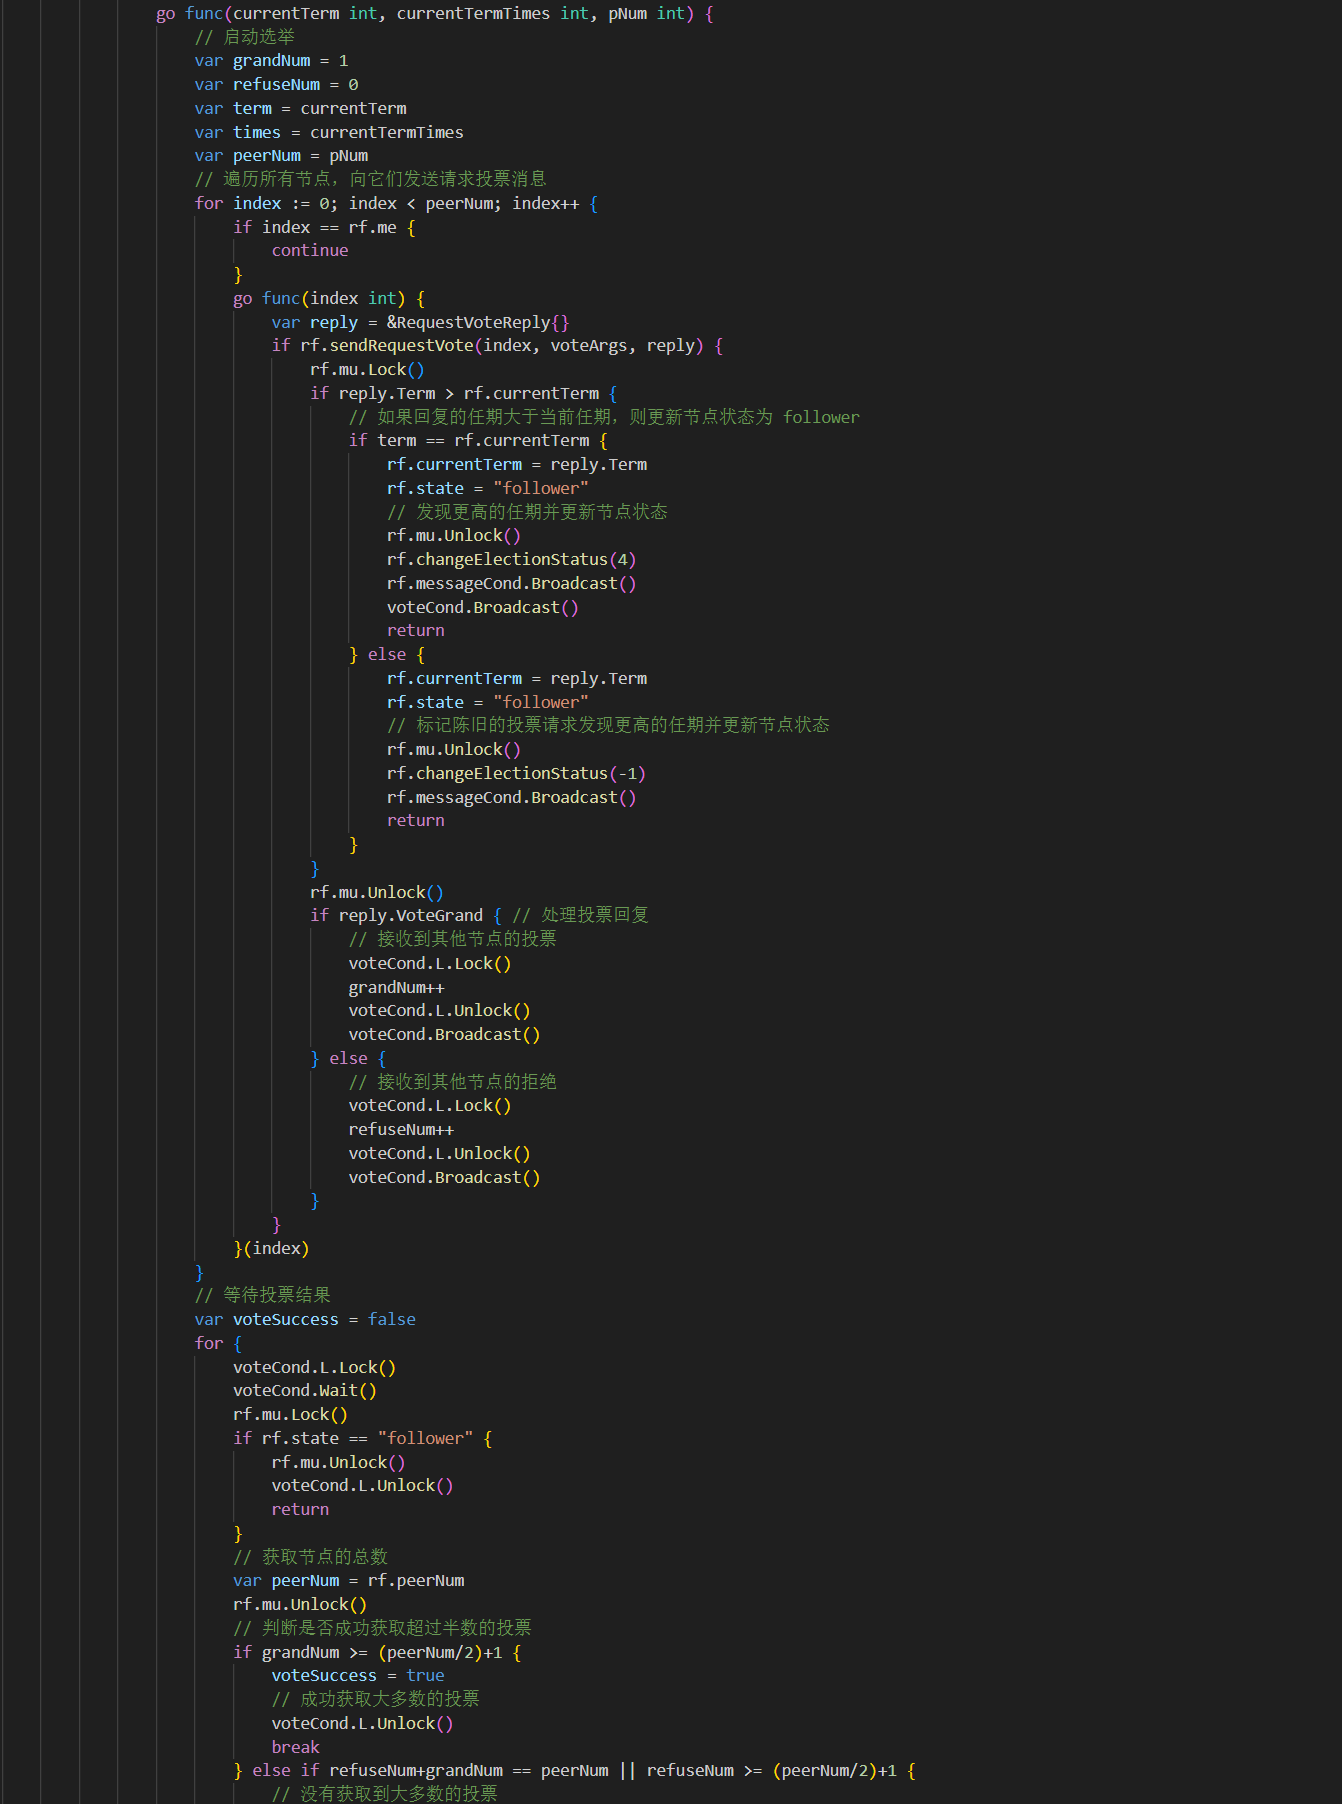
\includegraphics[height=1\textheight]{./2A/ticker2.png}
		\end{figure}
		\begin{figure}[H]
			\centering
			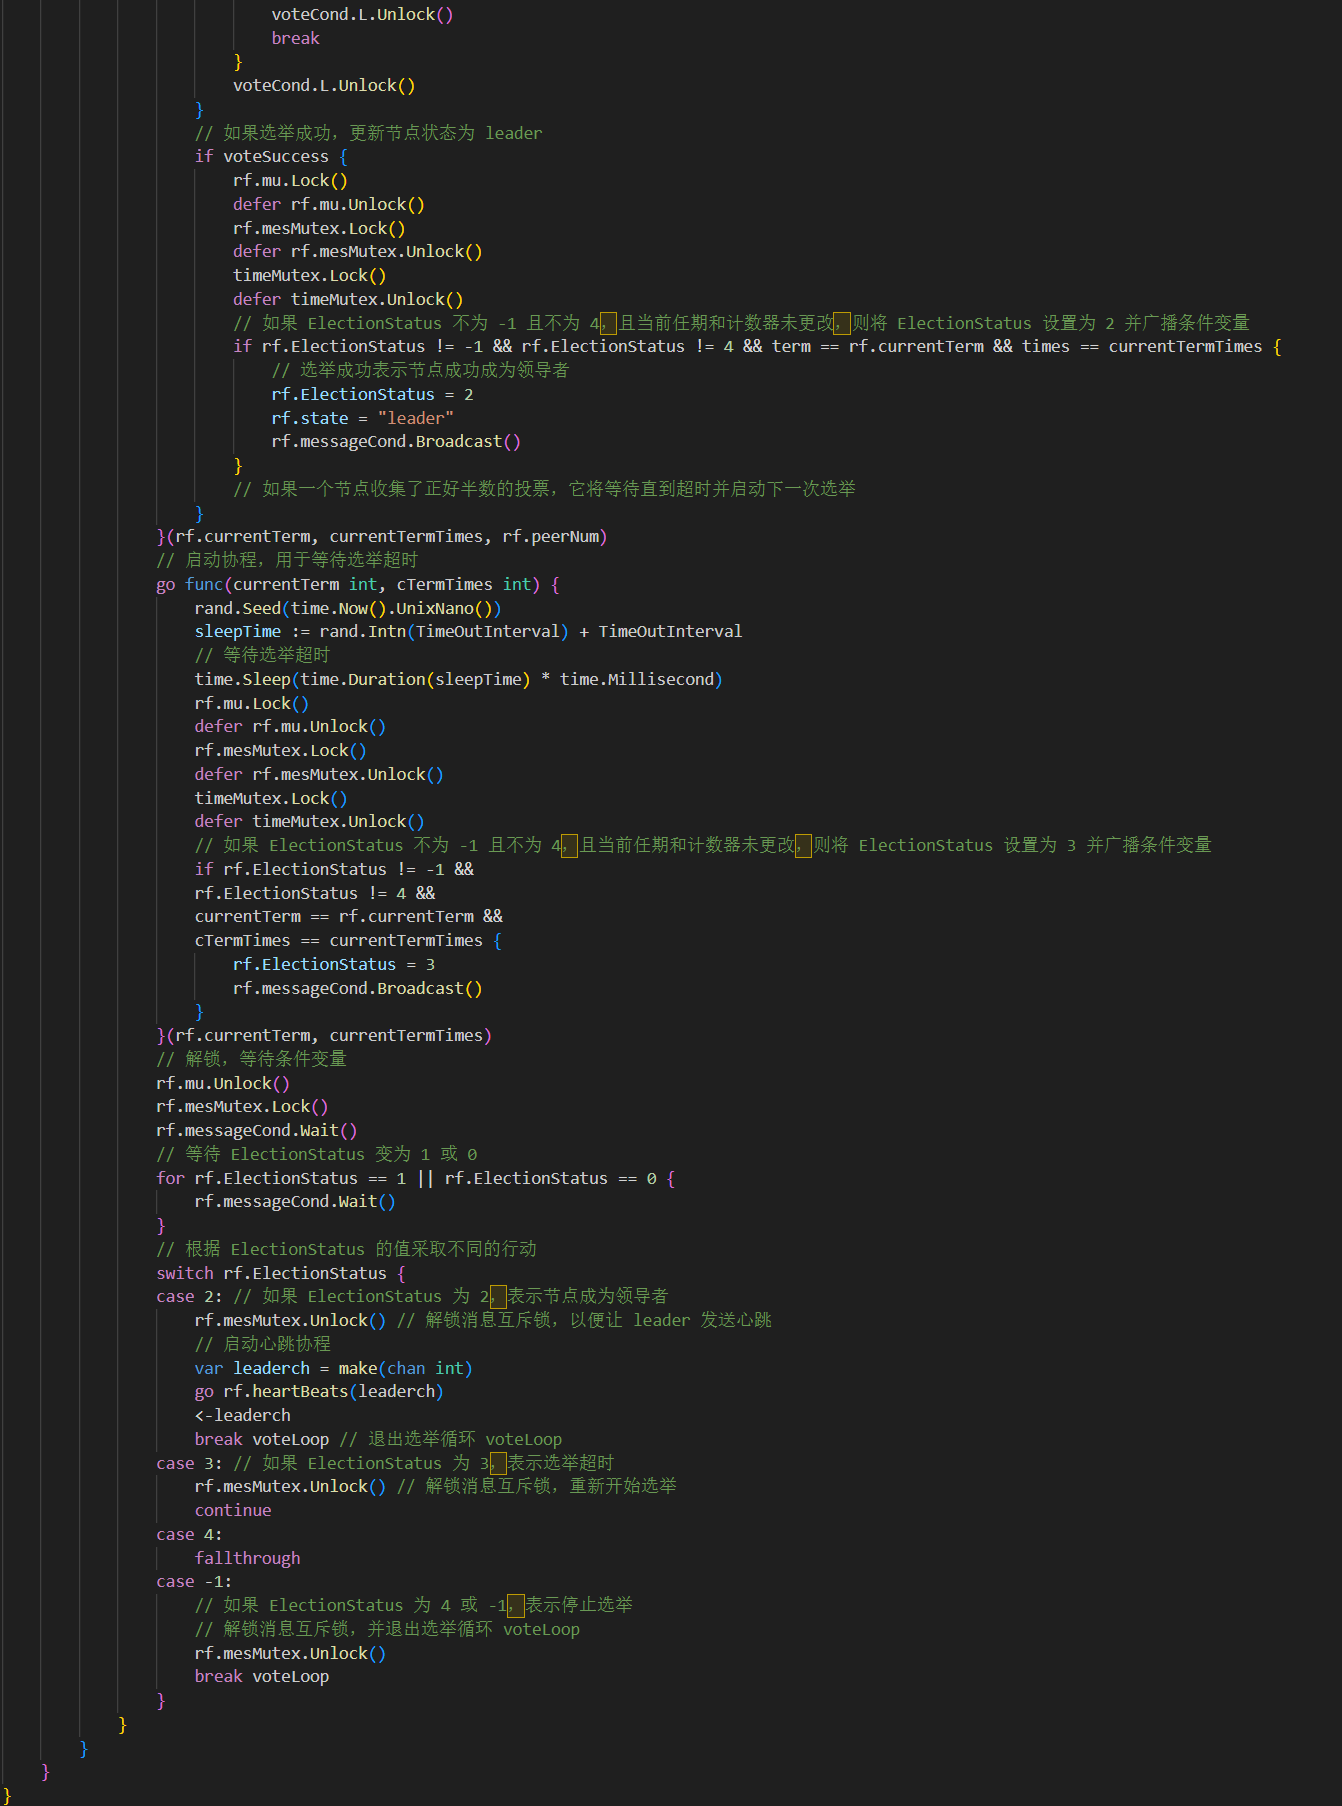
\includegraphics[height=0.95\textheight]{./2A/ticker3.png}
			\caption{ticker函数}
		\end{figure}
		\item 实现heartBeats函数
		\begin{figure}[H]
			\centering
			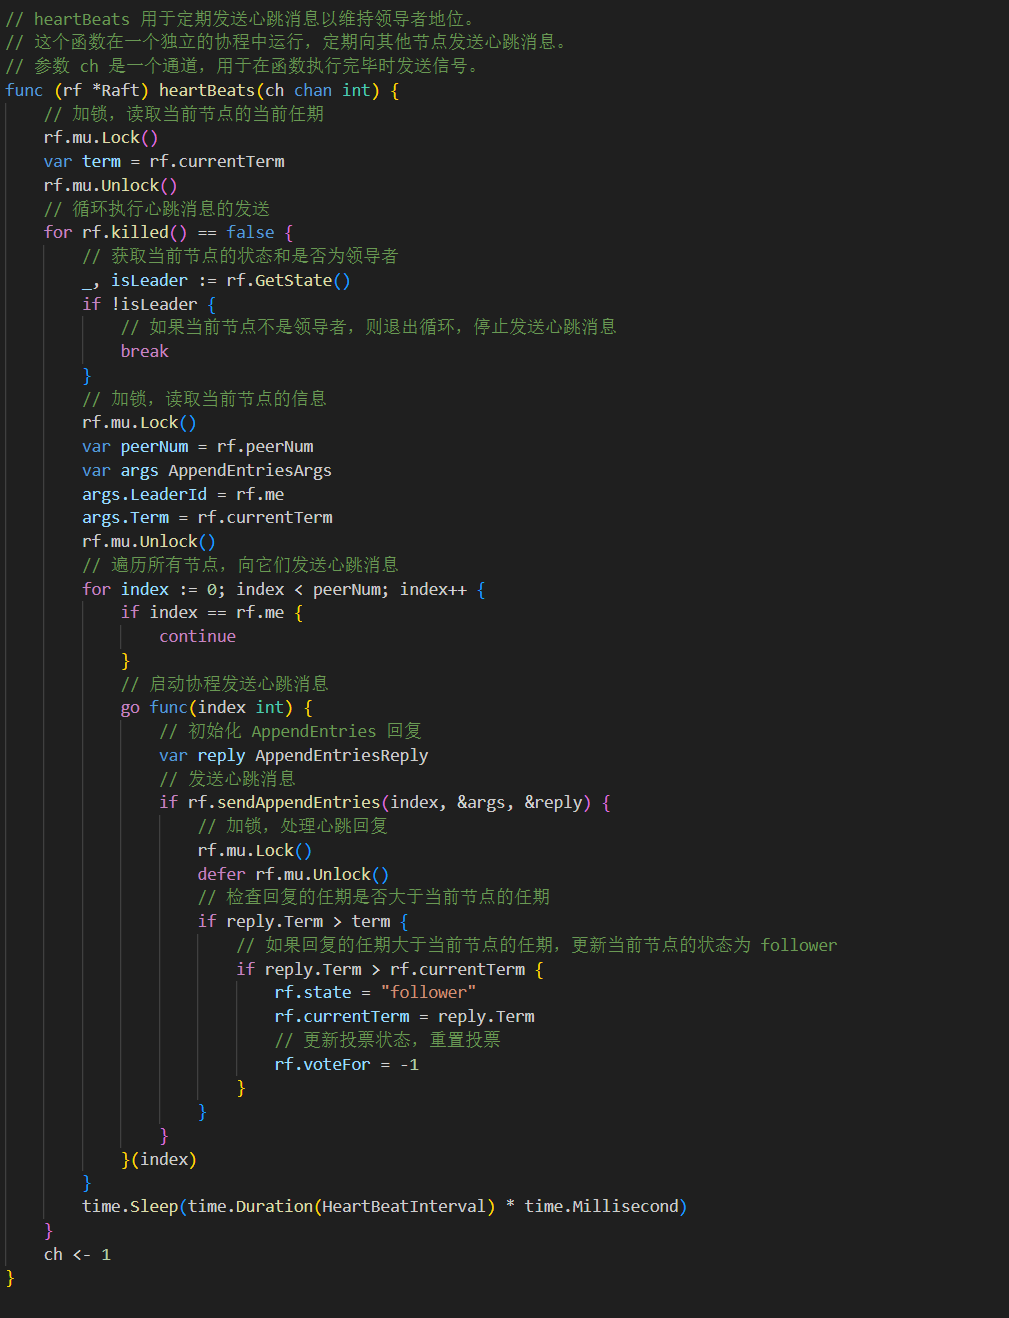
\includegraphics[height=0.92\textheight]{./2A/heartBeats.png}
			\caption{heartBeats函数}
		\end{figure}
		\item 完善Make函数
		\begin{figure}[H]
			\centering
			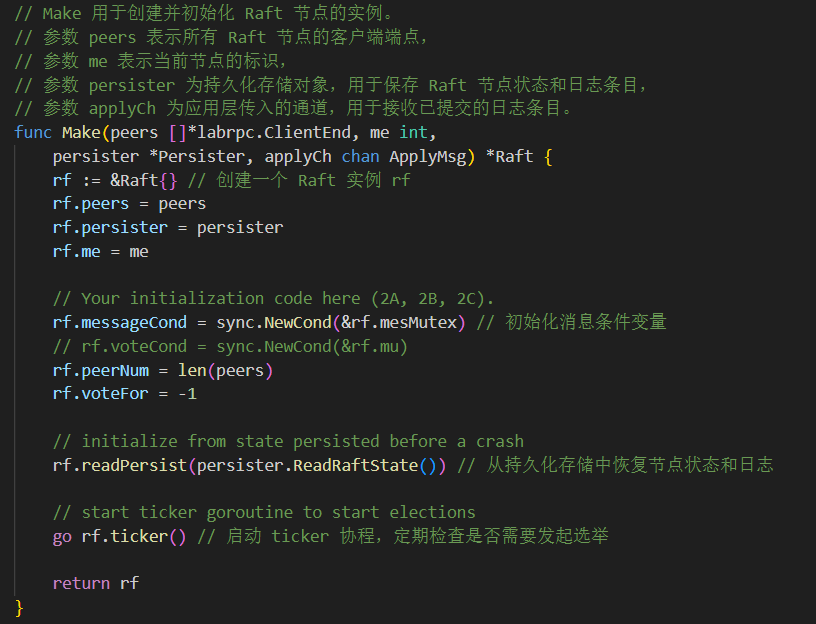
\includegraphics[width=0.8\textwidth]{./2A/Make.png}
			\caption{Make函数}
		\end{figure}
	\end{itemize}

	\subsection{测试结果}
	\begin{figure}[H]
		\centering
		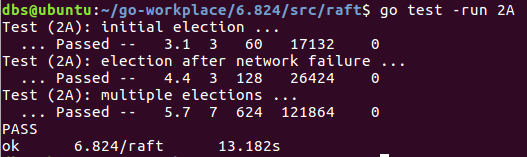
\includegraphics[width=0.8\textwidth]{./2A/2A result.png}
		\caption{2A运行结果}
	\end{figure}
	\begin{figure}[H]
		\centering
		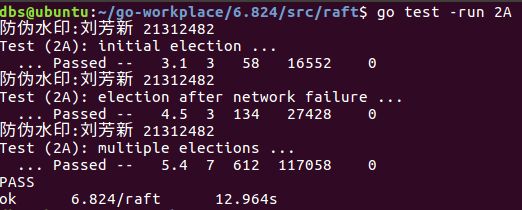
\includegraphics[width=0.8\textwidth]{./2A/2A result1.png}
		\caption{2A运行水印}
	\end{figure}
	\subsection{个人总结}
	在进行RPC调用时切勿持有锁,因为持有锁可能导致RPC调用期间的阻塞,从而阻塞其他活动。释放锁是至关重要的,因为在RPC调用结束后,可能发生了大量的事件,而调用期间的锁已经不再具有实际意义。举个例子:假设在term=5时发起了一个RPC调用来收集选票,当RPC返回并收集到足够的选票时,持有锁的节点检查状态时发现term=6。此时不能将节点变为Leader,因为此RPC的结果是让该节点成为term=5的Leader,而不是term=6的Leader。
	
	在进行RPC调用时,最好将其放在一个新开的协程中,以避免RPC的阻塞影响到协程的后续工作。例如,在投票阶段,候选者应该同时向其他Raft节点发起投票RPC。为了实现同时发起,每次投票RPC都应该由一个新的协程负责处理,否则每向一个节点发起投票RPC,就必须等待该节点的响应后才能向下一个节点发起投票RPC。这种并发的设计可以提高系统性能,确保不会因为等待某个RPC调用而阻塞其他并发操作。
	
	\section{lab2-B log}
	\subsection{任务分析}
	Lab 2B 旨在实现 Raft 日志的复制与一致性,是一个相对核心且具有一定难度的部分。主要涉及到日志复制的过程,包括日志RPC的交互、写入过程以及错误纠正的处理。
	
	\begin{itemize}
		\item 日志复制:在 Raft 中,每个节点都维护一份日志,用于记录系统状态的变化。每个日志条目包含一个命令,代表对状态机的一次更新。节点通过相互之间的日志复制来确保各自的状态机保持一致。
		\item 一致性:日志的复制需要确保整个系统中所有节点上的日志都保持一致。领导者负责向其他节点发送日志条目,以确保它们的日志保持一致。一旦大多数节点确认接收了一个条目,它就被认为是已提交的,可以应用到节点的状态机中。
		
		\item 日志条目的传输和确认:Lab 2B 要求实现日志条目的传输和确认机制。领导者向其他节点发送日志条目,其他节点需要确认接收。这可能涉及到网络通信、消息传递和节点状态的管理。
		
		\item 提交和应用:一旦一个日志条目被大多数节点确认接收,它就被视为已提交。在此之后,领导者会通知其他节点将已提交的日志应用到它们的状态机中,以保持整个系统的状态一致。
	\end{itemize}

	通过实现这些关键功能,Lab 2B 旨在确保 Raft 系统的日志同步、一致性和正确性。这涉及到处理复杂的分布式系统场景,对节点之间的通信和状态管理有着高要求。
	\subsection{功能设计}
	\subsubsection{实现LogEntry结构体}
	在进行 log 结构体的设计时,需要确保能够保存 Command,同时记录该日志对应的 index 和 term。并且,为了灵活处理不同数据类型的 Command,可以使用 interface\{\},类似于 ApplyMsg 结构体中对 Command 的设计。
	\subsubsection{实现Start函数}
	\texttt{Start()} 作为一个接口提供给外界,用于向 Raft 节点发送指令并请求其执行。下面是该函数的执行流程:
	
	\begin{enumerate}
		\item 函数收到一个命令时,首先判断自身是否为 Leader。若不是,则返回;若是,则继续执行下一步。
		
		\item Leader 收到命令后,需要将该命令保存到本地的日志中,并更新 \texttt{matchIndex}、\texttt{nextIndex}、\texttt{lastLogIndex}、\texttt{lastLogTerm} 等变量。
		
		\item 启动多个 goroutine 并发地向其他 Follower 发起日志复制请求。在每个 goroutine 中,应注意尽量只使用当前协程的局部变量。如果需要使用共享变量,应使用局部变量保存此刻的共享变量值。例如,在负责日志复制的 goroutine 中,将 \texttt{rf.nextIndex[id]} 这个共享变量的值赋给了局部变量 \texttt{nextIndex}。如果需要获取发起 goroutine 时的 \texttt{rf.currentTerm} 值,只需查看 \texttt{args.Term} 的值即可。
		
		\item 负责 Follower 编号为 $n$ 的节点的日志复制 goroutine 中,首先需要检查编号为 $n$ 的 Raft 节点的 \texttt{nextIndex}。将 \texttt{nextIndex} 和 \texttt{index} 进行比较,其中 \texttt{index} 为最新的日志的索引值。如果两者存在差值,说明 Leader 和编号为 $n$ 的 Raft 节点之间缺失了不止一个日志值,需要将 \texttt{nextIndex+1~index} 之间的日志也打包到日志数组中,一并发送给 Follower。随后,Leader 将 \texttt{nextIndex} 指定的索引号的日志包添加到日志数组中。
		
		\item Leader 继续将 \texttt{nextIndex} 位置的日志打包到日志数组中,然后通过 \texttt{sendAppendEntries} RPC 调用将日志数组发送给 Follower。如果该 RPC 调用返回值为 \texttt{true},表明日志同步成功,随后更新 \texttt{matchIndex[id]} 即可。在更新时,每个 goroutine 需要注意自身是否已经过时。如果一个 goroutine 想要将 \texttt{matchIndex[id]} 更新为 $n$,但是发现 \texttt{matchIndex[id]} 的数值大于 $n$,则表明该 goroutine 已经过时,不再更新 \texttt{matchIndex[id]} 的值。
	\end{enumerate}
	
	若该 RPC 调用返回值为 \texttt{false},则需要分情况进行处理:
	
	\begin{itemize}
		\item 如果 \texttt{reply.Term > args.Term},表明该 goroutine 已经过时,需要停止该 goroutine 并检查 Raft 节点是否及时更新了 \texttt{Term} 值。若没有,则将 \texttt{rf.currentTerm} 更新为 \texttt{reply.Term}。
		
		\item 如果 \texttt{reply.Term <= args.Term},表明 Follower 发现 \texttt{preLogTerm} 和 \texttt{preLogIndex} 不匹配,需要 Leader 发送更早的日志。这种情况下,Leader 可以逐步一个个地将前面的日志加入,并与 Follower 进行确认是否匹配。然而,一个个添加日志并询问 Follower 效率较低。应该利用 \texttt{reply} 中 Follower 的 \texttt{term} 值来加速定位,因为 Follower 中的日志的 \texttt{term} 值一定都不会大于 Follower 的 \texttt{term} 值。因此,那些 \texttt{term > follower.term} 的日志必然是 Follower 缺失的。随后尝试一个个添加更早的日志,直到 Follower 返回 \texttt{true},表示找到了两者日志相同的地方,并将后续的日志都同步上了。
	\end{itemize}
	
	Leader 完成了对一个 Follower 的同步后,进行 \texttt{matchIndex} 检查,确定是否有新的日志已同步到大多数节点上。该检查通过收集各个节点的 \texttt{matchIndex},对 \texttt{matchIndex} 出现的次数进行计数,形成一个键值对数组,其中键为 \texttt{matchIndex},值为达到此 \texttt{matchIndex} 的节点数量。该数组按键从高到低排序,然后遍历数组进行累加值,直到值累加的值刚好超过 Raft 节点数的一半,此时的键值即为此刻半数以上节点都已同步的最新日志的索引值。
	
	将这个索引值与 \texttt{commitIndex} 进行比较,若大于则表明有新的日志同步到半数以上节点,可以进行提交。随后更新 \texttt{commitIndex} 值,并将提交的指令发送到 \texttt{applyCh} 管道中,同时更新 \texttt{lastApplied} 变量的值。
	
	\subsubsection{继续完善AppendEntries函数}
	由于在Lab2B中,AE RPC调用不再仅仅是心跳(heartbeat),因此,我在这里将日志复制(log replication)和心跳两者进行了区分处理。在心跳时,调用 \texttt{AppendEntries} 时传递的参数中是没有日志数组的;而在进行日志复制时,必然会发送带有日志数组的参数。因此,我将此作为区分点。
	
	以下是这个函数的处理流程:
	
	\begin{enumerate}
		\item Term的比较以及对应的处理,在Lab 2A中已经讲述,此处不赘述。
		
		\item 若 \texttt{args.Entries} 数组为 \texttt{nil},那么表明为心跳调用;反之,表明为日志复制调用。
	\end{enumerate}
	
	\noindent \emph{心跳调用的 \texttt{AppendEntries} 时}:
	
	如果 \texttt{args.LeaderCommit > rf.commitIndex},则更新 \texttt{rf.commitIndex = args.LeaderCommit},并进入步骤2。反之返回 \texttt{true}。
	
	更新了 \texttt{rf.commitIndex} 表明有新的日志可以提交并执行了。随后,将那些日志发送到 \texttt{applyCh} 管道中,并更新 \texttt{lastApplied} 变量的值。\\
	
	
	\noindent \emph{日志复制调用的 \texttt{AppendEntries} 时}:
	
	日志同步应该从双方日志一致的索引点开始,因此这里着重点在于反馈给 Leader 一致的索引在哪里。当然,里面还有很多特殊情况需要考虑。
	
	\begin{enumerate}
		\item Follower 需要检查发送来的 AE 包是否满足本节点的缺失情况,也就是检查 \texttt{args.PreLogIndex} 和 \texttt{rf.lastLogIndex}。
		
		\item 如果 \texttt{args.PreLogIndex > rf.lastLogIndex} 表明肯定不满足本节点的缺失情况,返回 \texttt{false};反之进入步骤3。
		
		\item 来到这儿表明 \texttt{args.PreLogIndex <= rf.lastLogIndex},这依旧不能确定这个 AE 包是否满足本节点的缺失情况,可能本节点存在部分无效的日志。例如,一个 Leader 加了很多日志,但是断开了连接,这些新加的日志都没有来得及发送给任何一个节点。后续重连回来就成为 Follower 了,那么这些独自拥有的日志就是无效日志。
		
		\item Raft 算法的特点之一是,如果两个日志的索引和任期都是一样的,那么这两个日志必然是一致的。因此,Follower 仅需判断 \texttt{args.PrevLogTerm == rf.log[args.PreLogIndex]} 是否成立。如果成立,表明,在 \texttt{args.PreLogIndex} 这里以及之前的日志都是同步的了。否则,就是 \texttt{args.PreLogIndex < rf.lastLogIndex},但是这个索引值为 \texttt{args.PreLogIndex} 处的日志,两个节点的日志依旧不一致,需要返回 \texttt{false},让 Leader 继续往前找到一致的索引。
		
		注意:Follower 发现发来的这个 AE 包中的日志的 \texttt{PrevLogIndex} 和 \texttt{PrevLogTerm} 都是符合条件的,但是依旧不一定就要同步上来。需要注意部分 AE 是过时的,例如,1号 AE 包负责将 Follower 同步到索引 $n$ 处的日志;2号 AE 包负责而将 Follower 同步到索引 $n+1$ 处的日志。但是1号 AE 比2号还迟,2号 AE 包已经将各个 Follower 的日志同步到了索引 $n+1$ 处。当过时的1号 AE 包被 Follower 接收到时,Follower 依旧按照包中指示同步到索引 $n$ 处,那么同步进度就倒退了,将会引发 bug。因此,Follower 还需要检测这个 AE 是否过时。
		
		\item 到这里,表明这个 AE 包是合法的,同步的开始日志处,双方也都是一致的。但是需要判断这个 AE 是否是过时的。Follower 仅需检测,发来的 AE 包中,\texttt{args.Entries} 中最新的日志,本节点中是否存在。若存在,表明无需同步,这个包是过时的。若不存在则进入下一步进行同步。
		
		\item 更新本地的 \texttt{rf.log},\texttt{rf.lastLogIndex},\texttt{rf.lastLogTerm} 等变量。
	\end{enumerate}
	
	\subsubsection{继续完善heartBeats函数}
	在 heartBeats 函数中增加一个功能,即通知 follower 更新 commitIndex。值得注意的是,需要考虑到部分节点尚未同步日志。如果Leader无条件地通知那些 follower 自身的 commitIndex 已经更新,要求它们也同步更新,可能导致混乱。因此,领导者应该根据 follower 的情况来进行选择性的通知。
	
	Leader应该通知那些同步进度超过 commitIndex 的节点。Leader在 commitIndex 这个数组中记录了各个 follower 的同步进度,因此可以利用这个数组来进行判断。
	
	在本实验中,若Leader要通知节点更新 commitIndex,仅需在发给 follower 的 AE 包中赋值 args.LeaderCommit = rf.commitIndex,随后 follower 就能收到最新的 commitIndex。
	
	如果Leader发现节点的同步进度不够,并不通知节点进行更新 commitIndex,那么在发给 follower 的 AE 包中不赋值 args.LeaderCommit 即可。这个参数的默认值为 0,并不会对 follower 的 commitIndex 造成任何影响。
	\subsubsection{继续完善ticker函数}
	在本实验中,需要进行log replication,Leader需要使用nextIndex和matchIndex这两个变量,因此每个raft节点成为leader后都需要对这两个变量进行初始化。
	
	按照paper中的说法,leader开始需要将matchIndex数组全部初始化为0,nextIndex数组的初始化则按照自身的nextIndex初始化。
	\subsubsection{继续完善Make函数}
	根据实验说明,index 应当从 1 开始。为了使 index 的值和 log 数组的索引值对应起来,我使用一个 index 和 term 均为 0 的 log 占用了数组的 0 号索引位。这样的处理使得 index 为 1 的 log 存放在 log[1] 处,而非 log[0] 处。同时,这个 index 和 term 均为 0 的 log 作为数组的头部,可以在遍历 log 数组时用来判断是否到达数组的头部。
	
	applyCh 的值可以直接从 Make 函数的参数中获取并赋值。
	
	对于 nextIndex 和 matchIndex,由于它们都是切片,需要使用 make 进行初始化。此外,这些切片的长度应该和 Raft 节点数一样。
	
	\subsection{代码实现}
	\begin{itemize}
		\item 实现LogEntry结构体
		\begin{figure}[H]
			\centering
			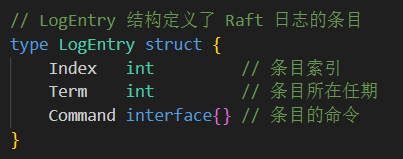
\includegraphics[width=0.8\textwidth]{./2B/LogEntry.png}
			\caption{LogEntry结构体}
		\end{figure}
		\item 实现Start函数
		\begin{figure}[H]
			\centering
			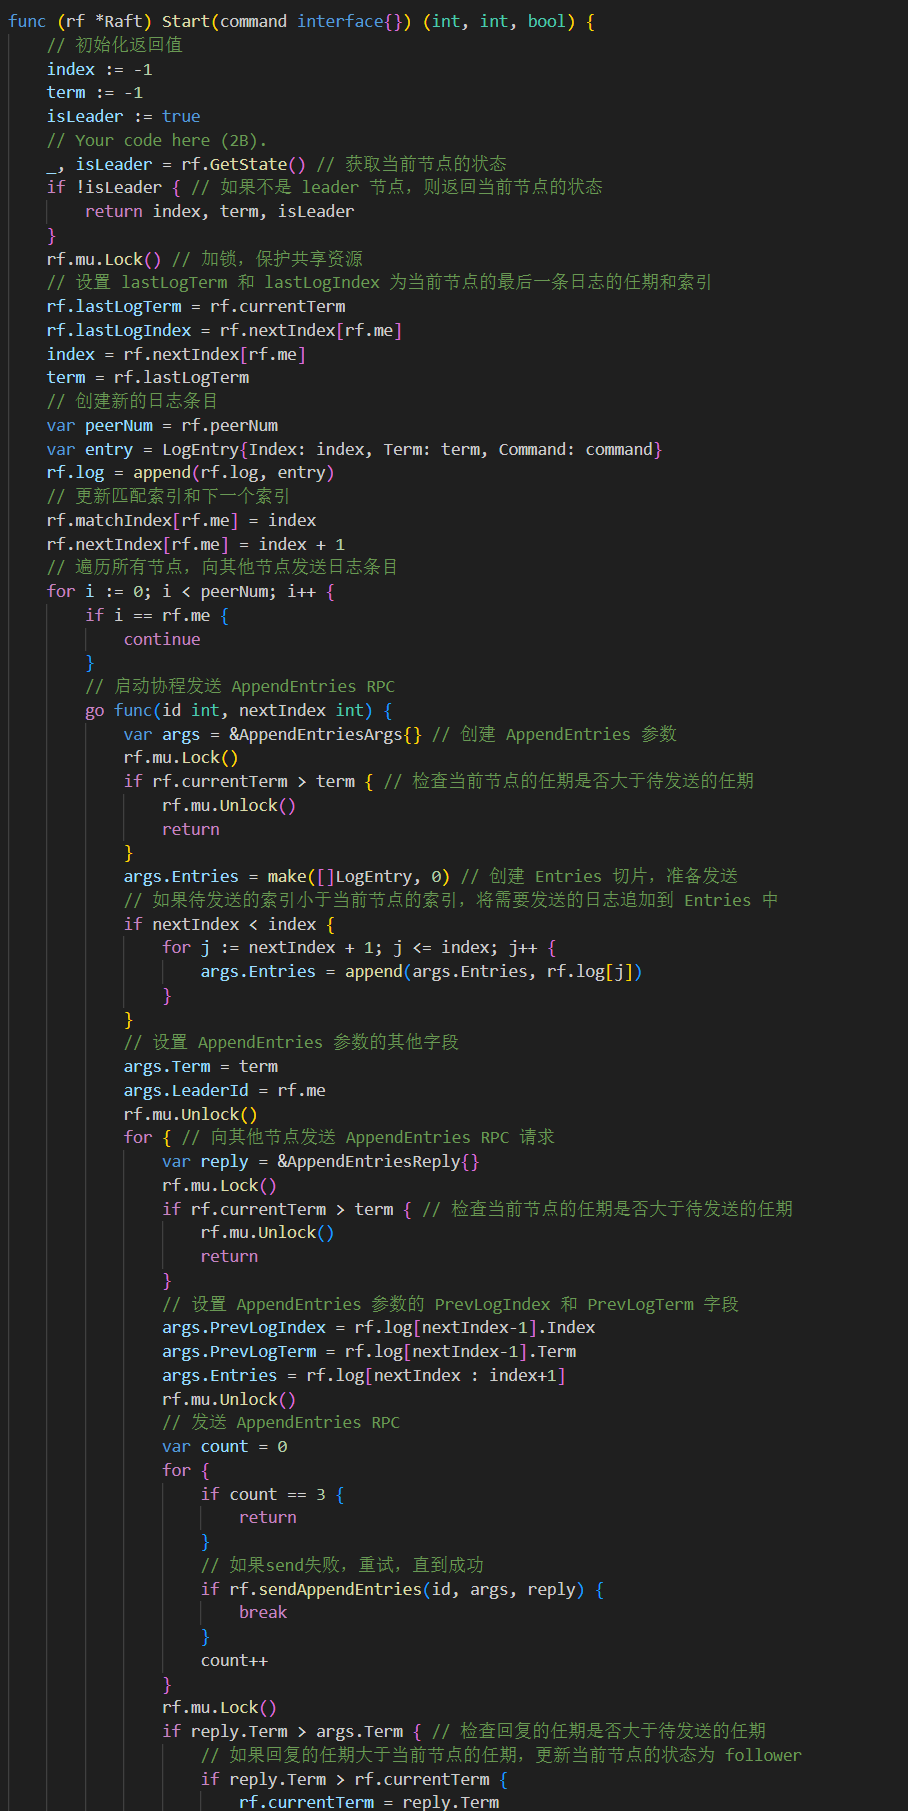
\includegraphics[height=1\textheight]{./2B/Start1.png}
		\end{figure}
		\begin{figure}[H]
			\centering
			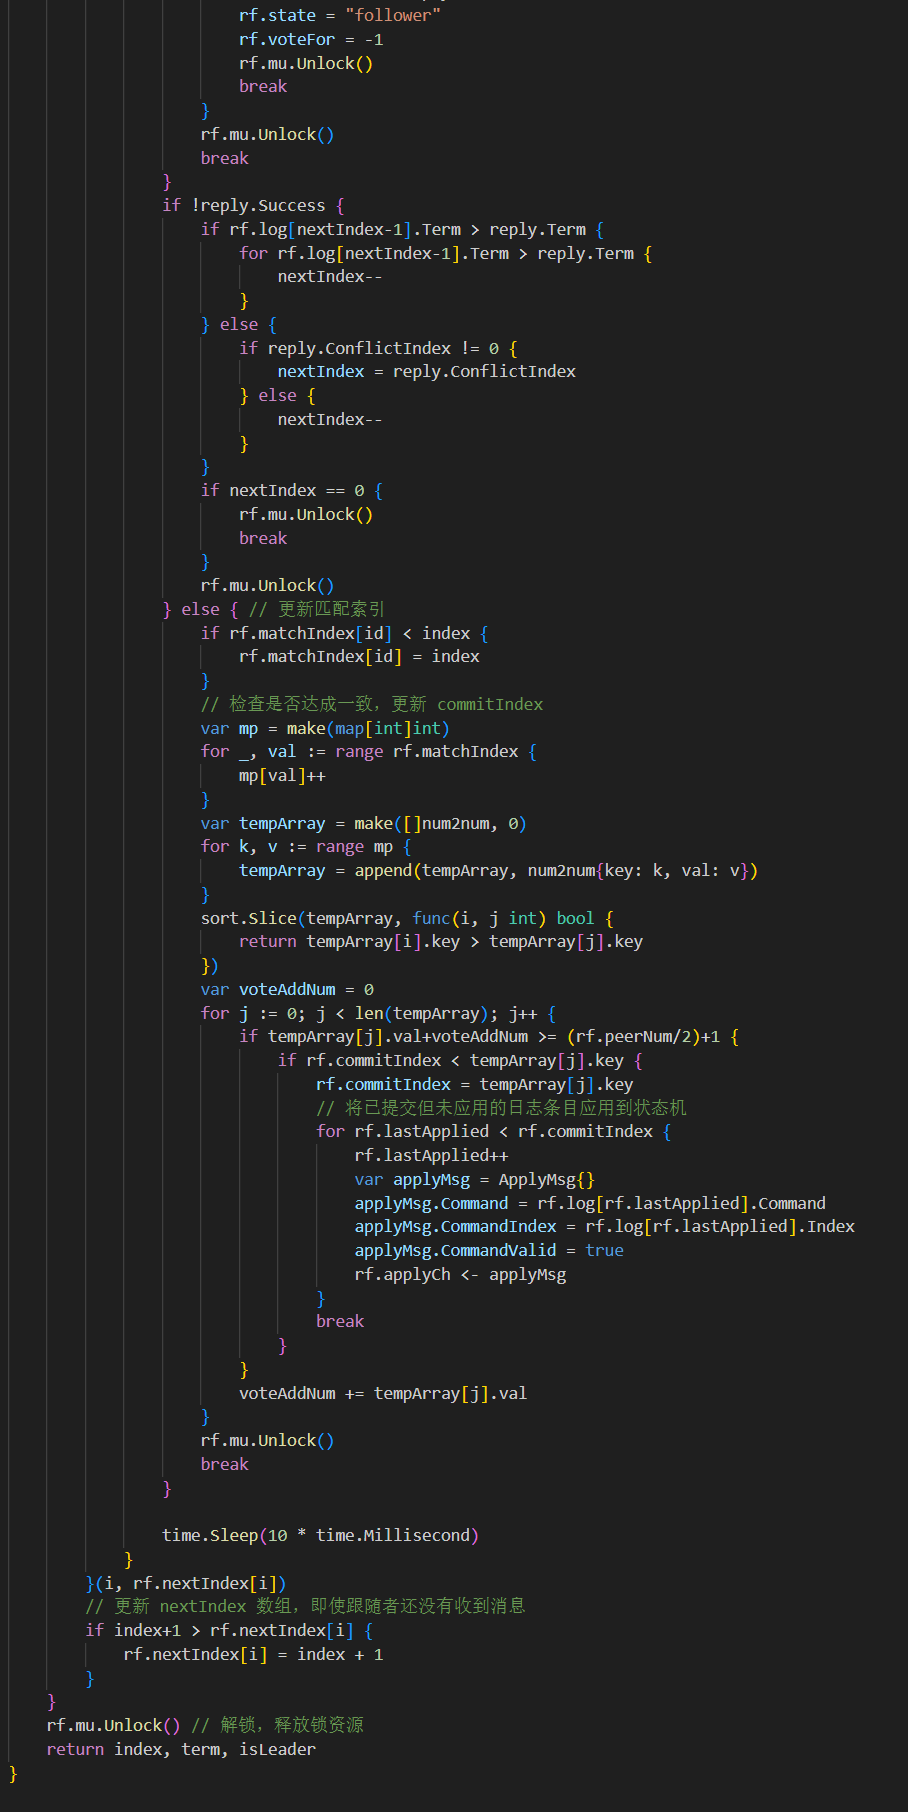
\includegraphics[height=0.95\textheight]{./2B/Start2.png}
			\caption{Start函数}
		\end{figure}
		\item AppendEntries函数
		\begin{figure}[H]
			\centering
			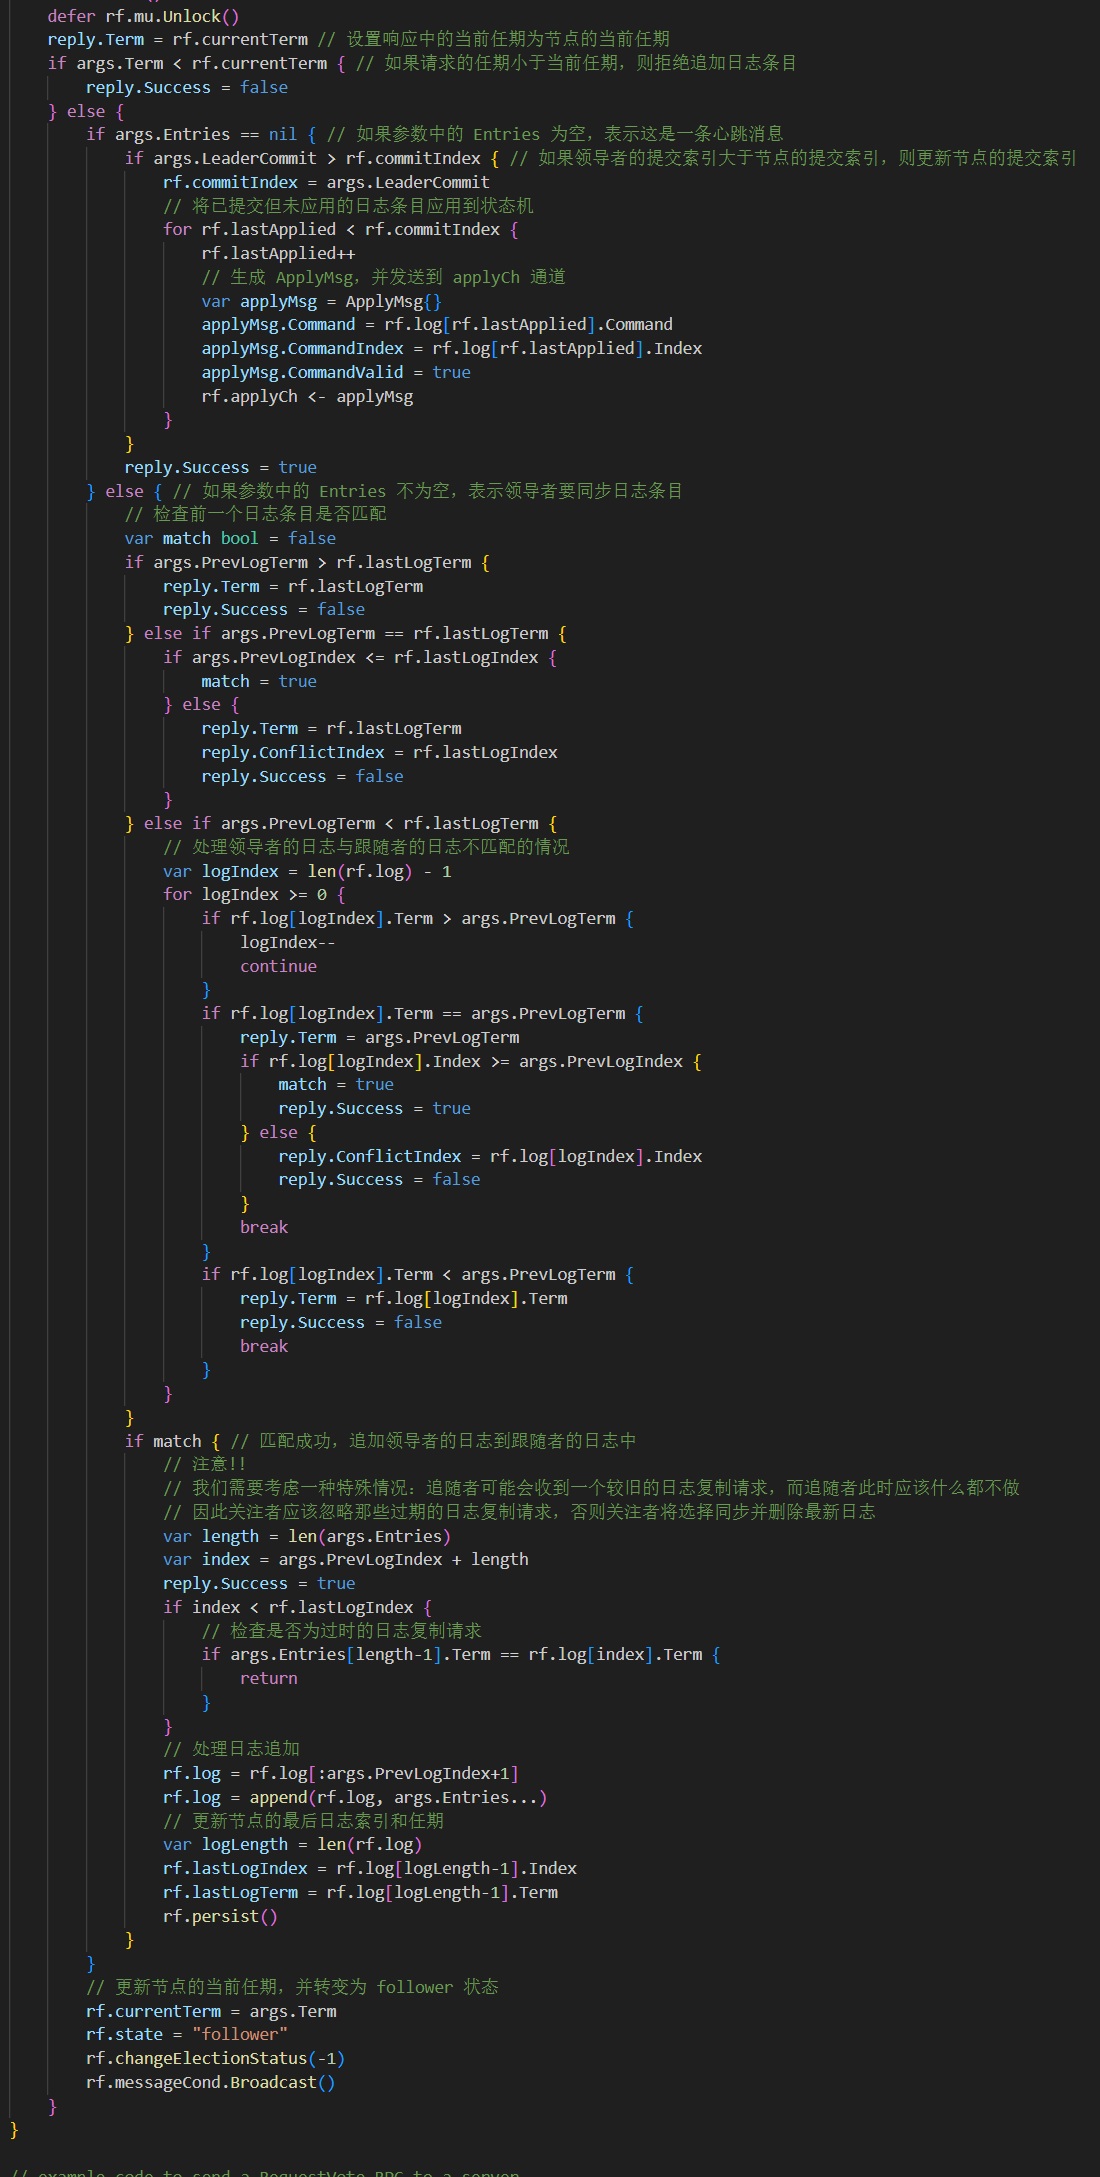
\includegraphics[height=0.9\textheight]{./2B/AppendEntries.png}
			\caption{AppendEntries函数}
		\end{figure}
		\item heartBeats函数
		\begin{figure}[H]
			\centering
			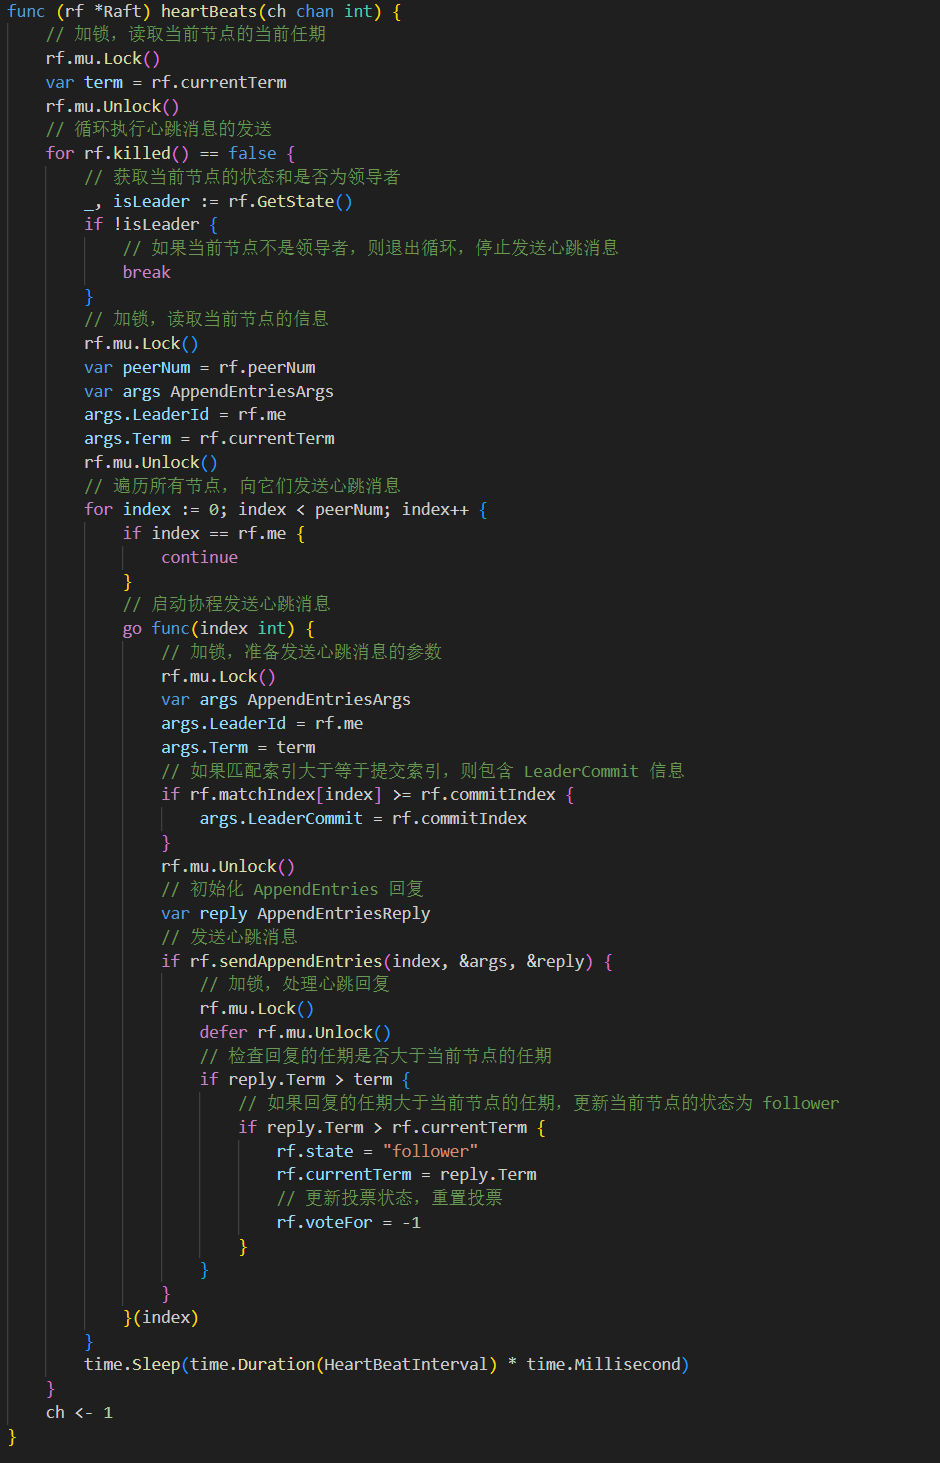
\includegraphics[height=0.9\textheight]{./2B/heartBeats.png}
			\caption{heartBeats函数}
		\end{figure}
		\item ticker函数
		\begin{figure}[H]
			\centering
			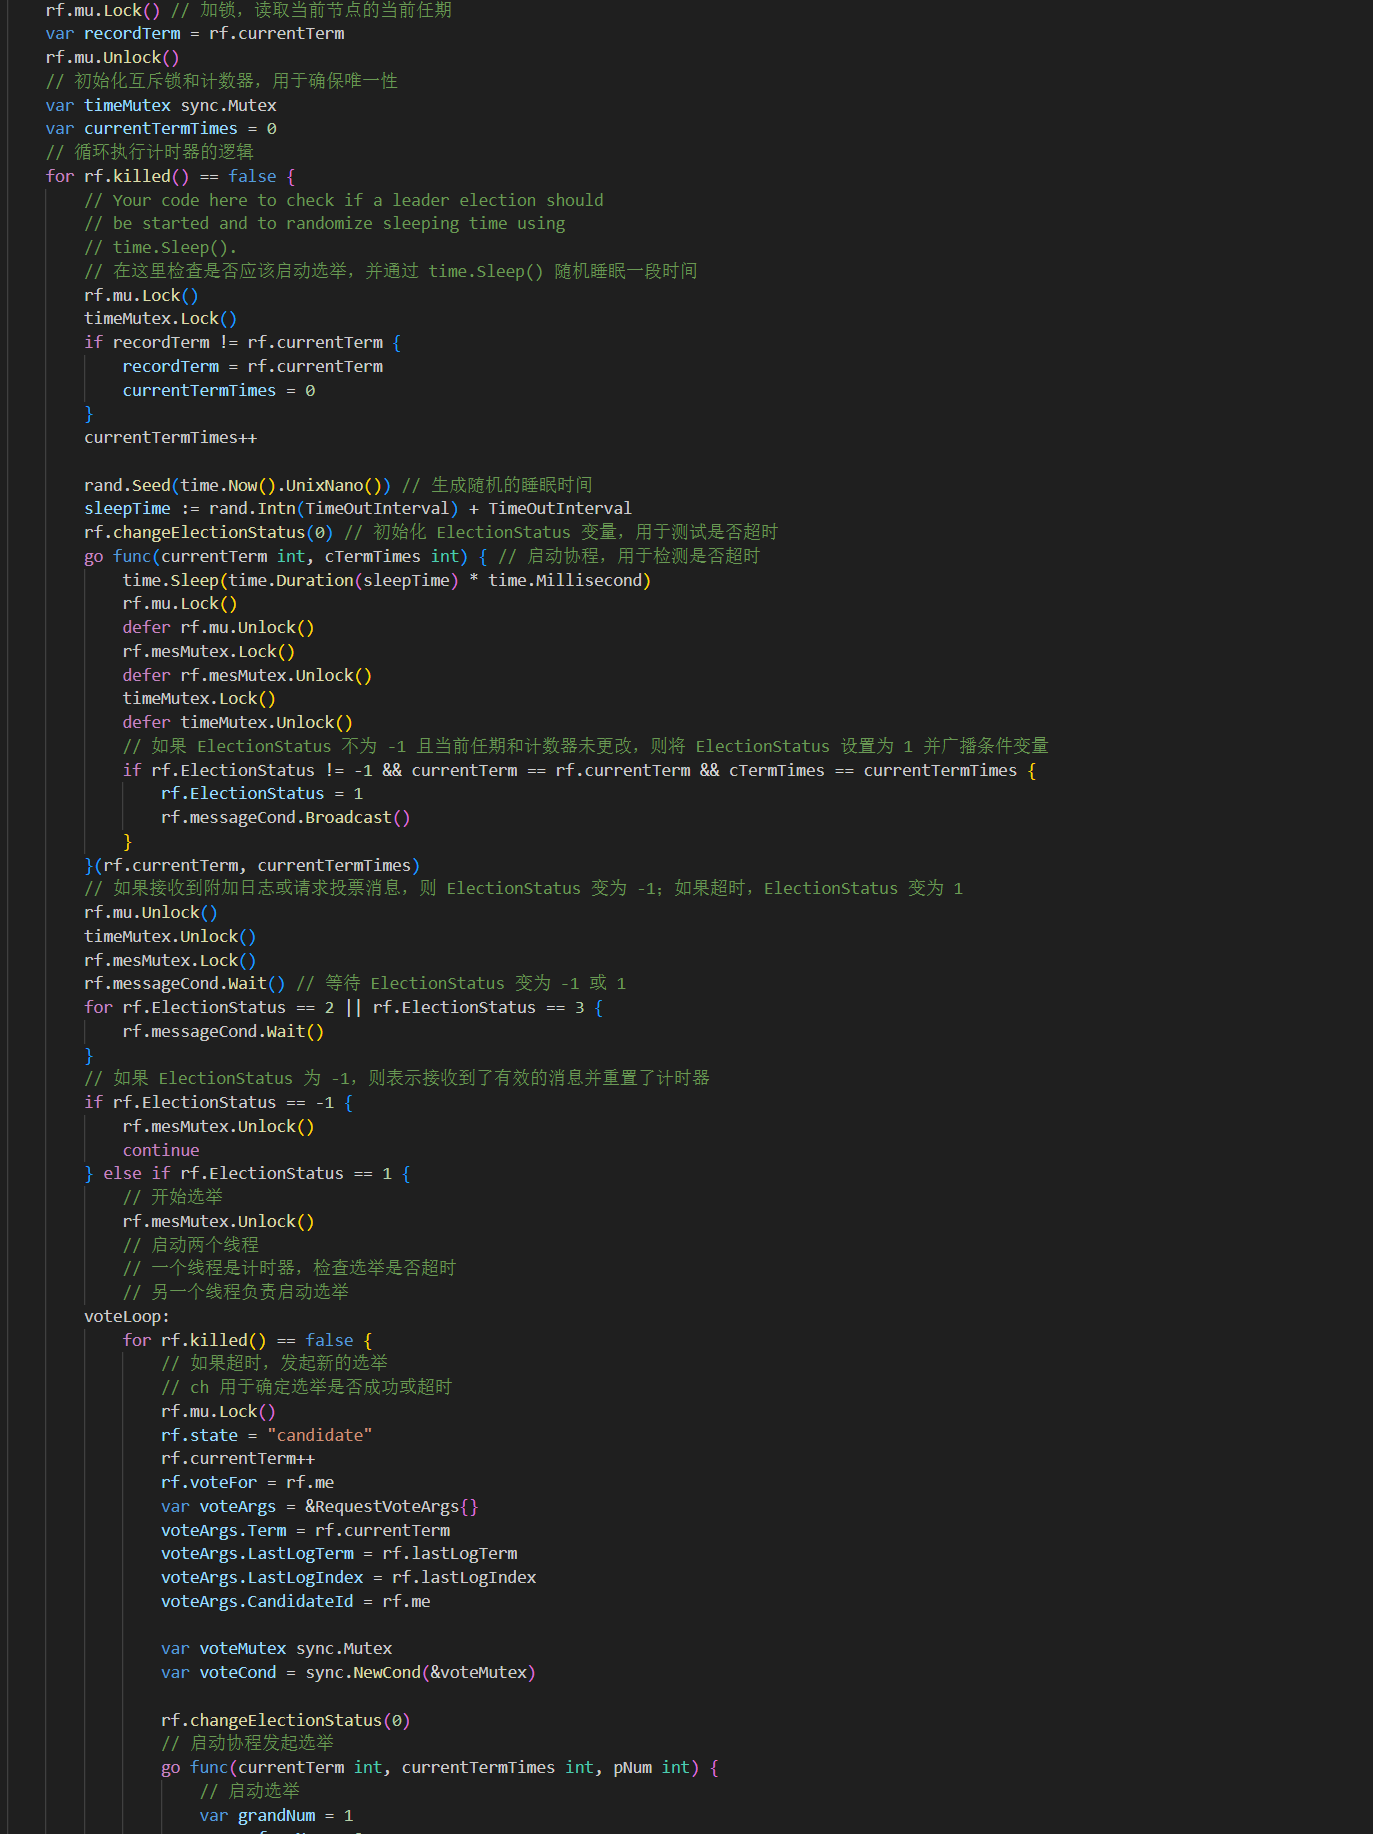
\includegraphics[height=0.9\textheight]{./2B/ticker1.png}
		\end{figure}
		\begin{figure}[H]
			\centering
			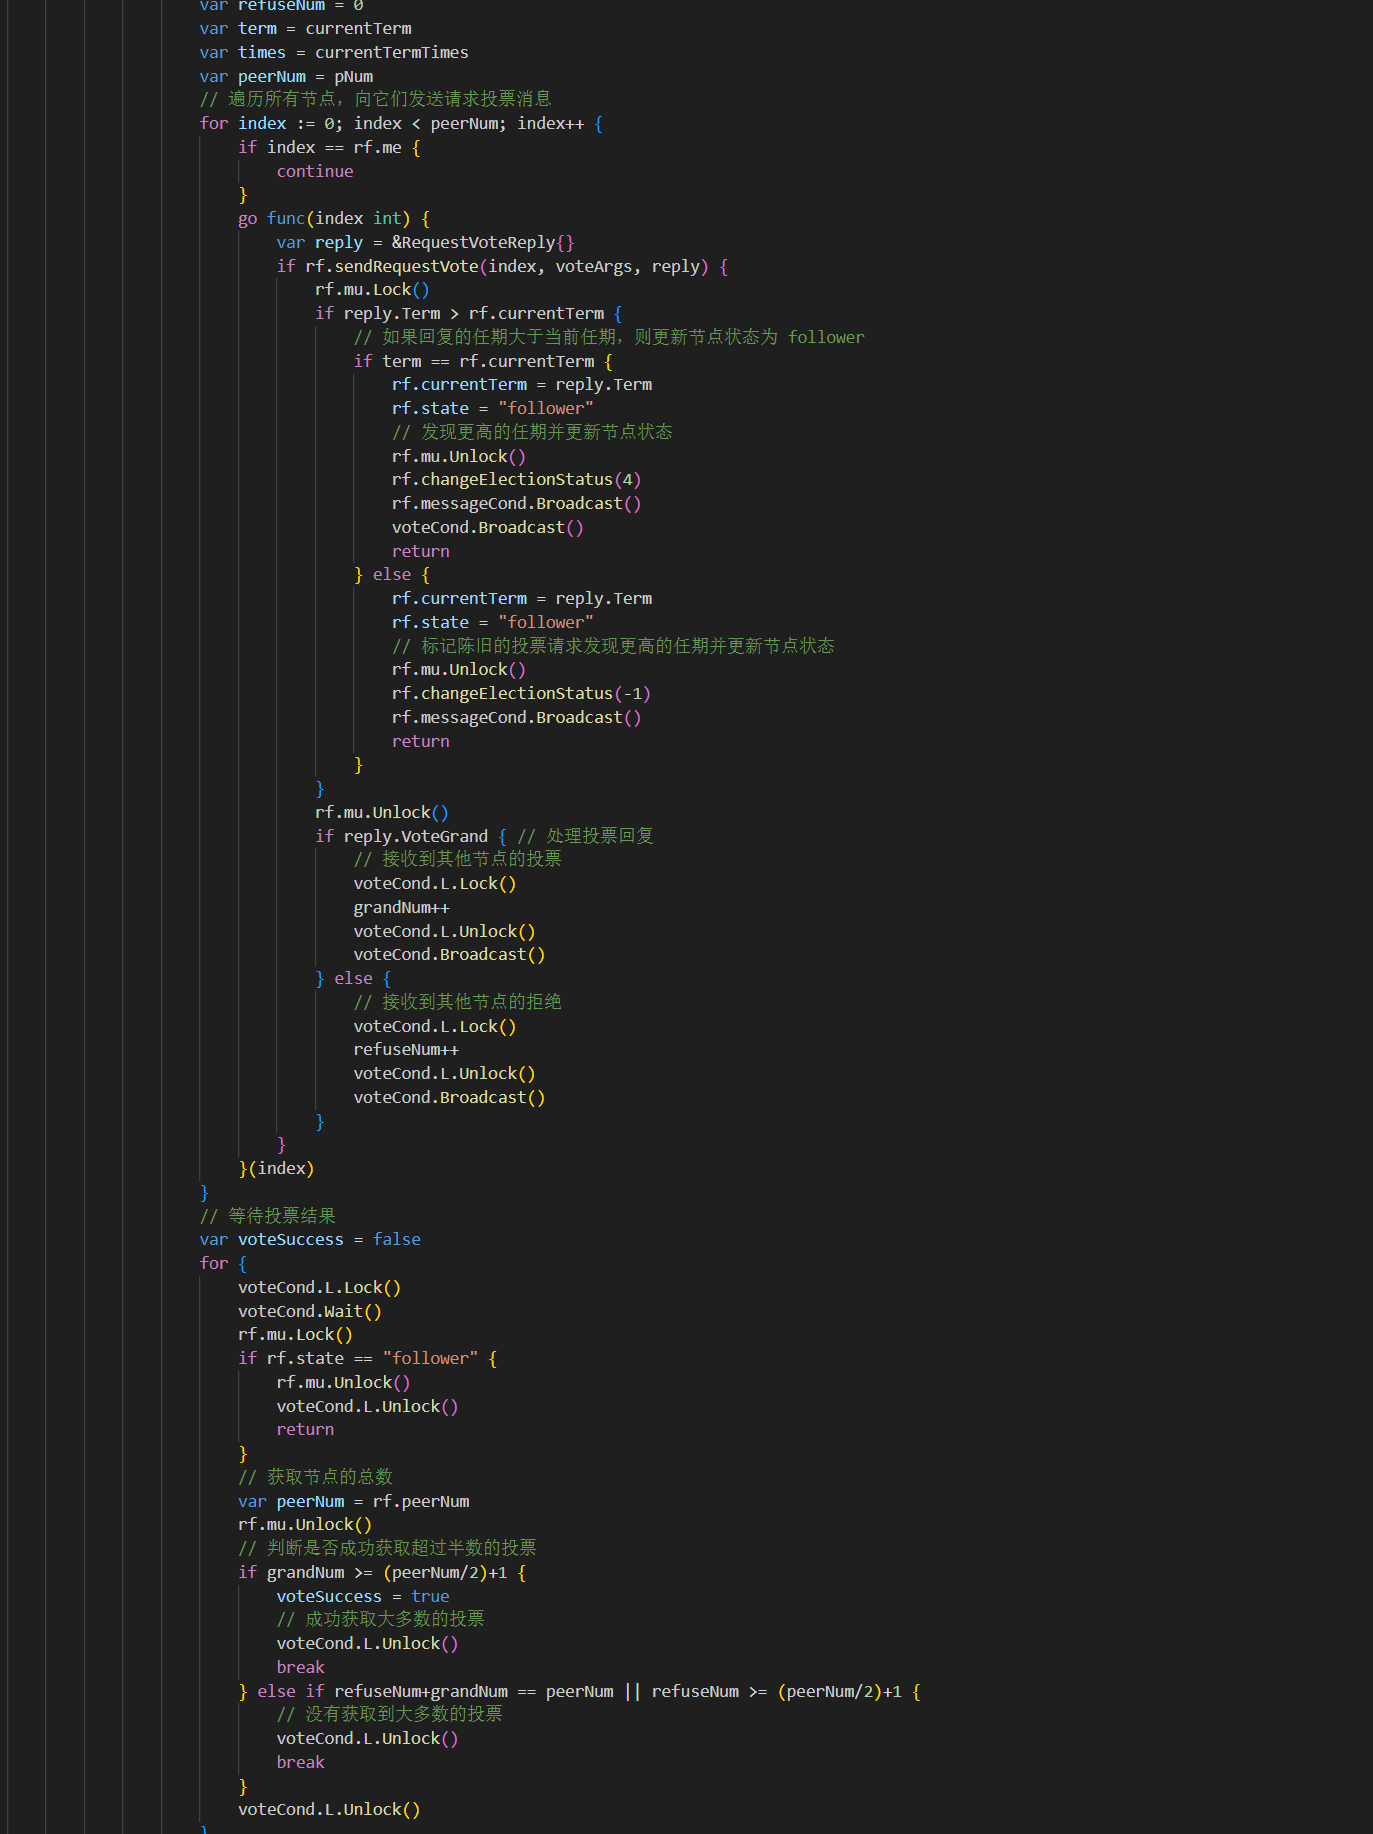
\includegraphics[height=1\textheight]{./2B/ticker2.png}
		\end{figure}
		\begin{figure}[H]
			\centering
			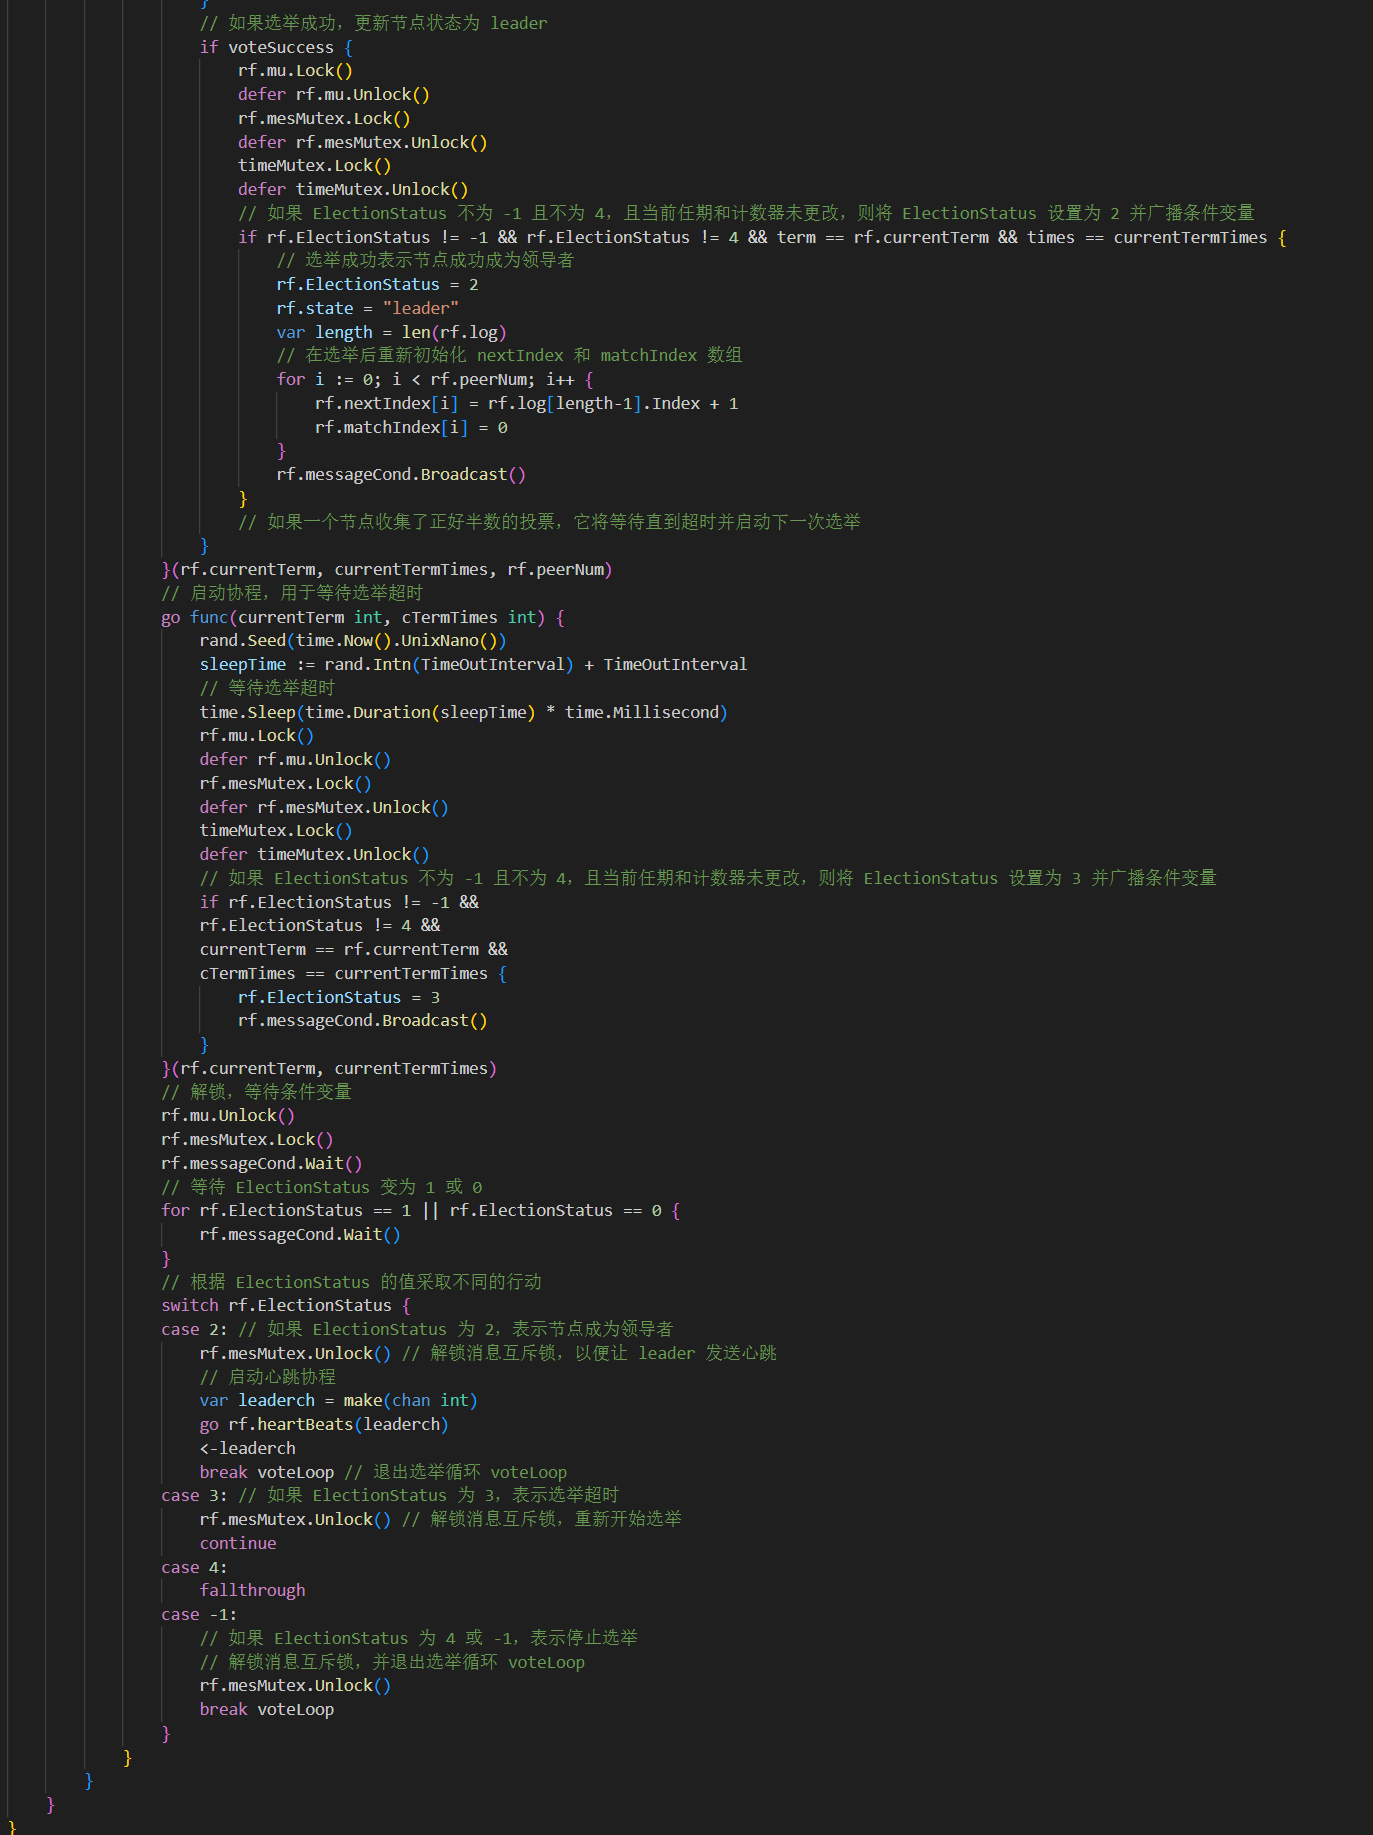
\includegraphics[height=0.95\textheight]{./2B/ticker3.png}
			\caption{ticker函数}
		\end{figure}
		\item Make函数
		\begin{figure}[H]
			\centering
			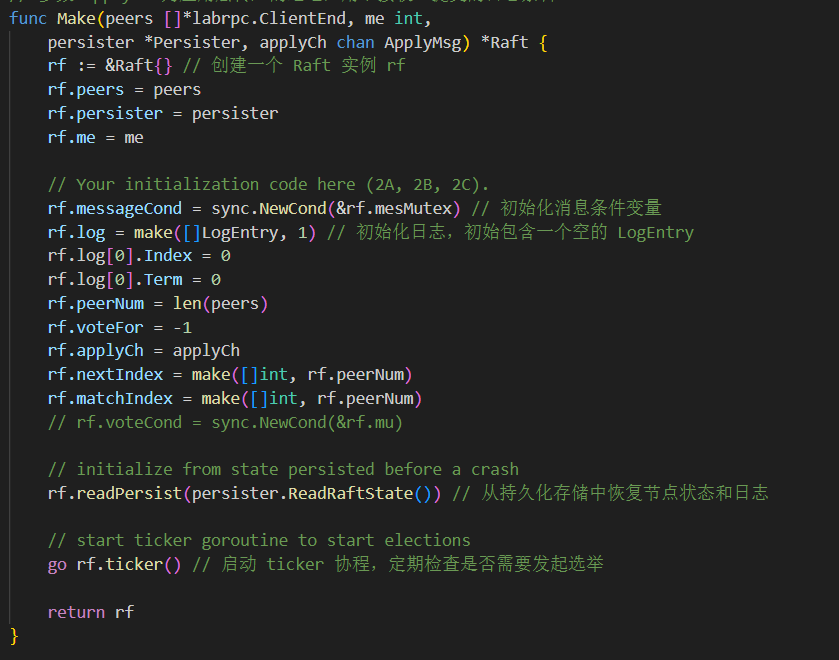
\includegraphics[width=0.8\textwidth]{./2B/Make.png}
			\caption{Make函数}
		\end{figure}
	\end{itemize}
	
	\subsection{测试结果}
	\begin{figure}[H]
		\centering
		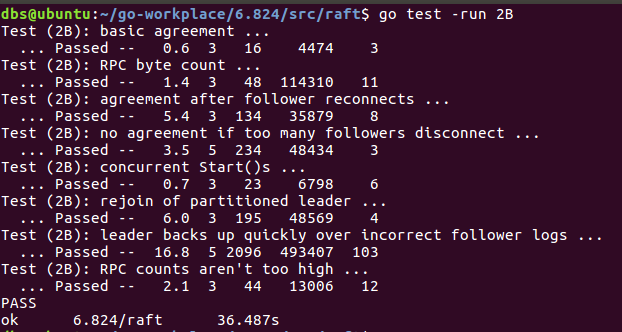
\includegraphics[width=0.8\textwidth]{./2B/2B result.png}
		\caption{2B运行结果}
	\end{figure}
	\begin{figure}[H]
		\centering
		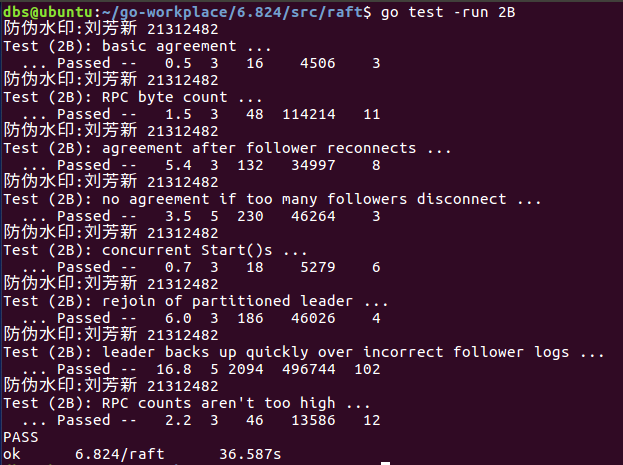
\includegraphics[width=0.8\textwidth]{./2B/2B result1.png}
		\caption{2B运行水印}
	\end{figure}
	
	\subsection{个人总结}
	在写2B的过程中,我找到了之前2A写的一些bug,在处理多线程程序时,确实存在一些比较隐蔽的bug,尤其是涉及到锁的使用和线程同步的情况。死锁是其中一个比较棘手的问题,因为它可能在程序运行的某个点触发,而不一定在每次运行都表现出来。可能突然某次运行就有一个raft节点发生卡死,没有任何响应了,大概率是因为锁设置的太多了,导致某处出现了死锁。因此我的经验是:
	
	减少锁的使用: 尽量减少对共享资源的锁定,可以考虑使用更细粒度的锁,或者使用无锁的数据结构。过多的锁可能导致竞争条件,增加了死锁的概率。
	
	避免嵌套锁: 当一个线程持有一个锁的同时尝试获取另一个锁,容易导致死锁。确保在获取锁的时候,尽量避免嵌套锁的情况。
	
	\section{lab2-C persistence}
	\subsection{任务分析}
	Lab 2C的任务是对Raft一致性算法中的关键状态信息进行持久化处理。这一操作的主要目的在于确保系统能够在节点重启或发生故障时从持久化存储中进行恢复,以维持一致性。以下是对Lab 2C任务的详细分析:
	\begin{itemize}
	\item 持久化的状态信息:在Raft中一些至关重要的状态信息,需要被持久化存储,以确保在节点重启后能够正确继续运行。这些信息包括日志(Log)、当前任期(term)以及投票对象(votedFor)。
	
	\item 存储和恢复逻辑: 在Lab 2C实验中,并非直接存储于磁盘,而是通过一个代表性的 Persister 对象来完成。这个对象充当了持久化存储的代理,负责处理状态信息的存储和恢复逻辑。
	
	\item 一致性保障: 通过持久化状态信息,Lab 2C实验确保了在节点重启后系统能够正确继续运行,而不会发生数据丢失或不一致的情况。这种机制提供了强有力的一致性保障,增强了系统的可靠性和稳定性。
	\end{itemize}

	\subsection{功能设计}
	\subsubsection{完善persist函数}
	这个函数就是把节点必要的信息进行持久化保存,按照所给出的示例代码,以及论文上的描述即可写出来。
	\subsubsection{完善readPersist函数}
	这个函数就是把之前保存的信息重新读取并加载给节点,不过不能仅仅只是把需要持久化的那几次状态给恢复了。例如,我们这里持久化了currentTerm、voteFor、log。但是我们恢复过程中,可以通过log信息来恢复节点的lastLogTerm以及lastLogIndex,这两个信息也需要恢复,不然就会出现问题。
	\subsection{代码实现}
	\begin{itemize}
		\item 完善persist函数
		\begin{figure}[H]
			\centering
			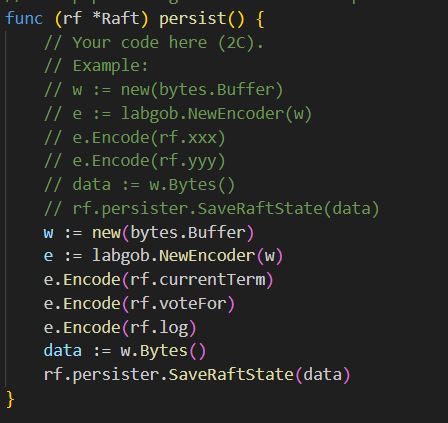
\includegraphics[width=0.65\textwidth]{./2C/persist.png}
			\caption{persist函数}
		\end{figure}
		\item 完善readPersist函数
		\begin{figure}[H]
			\centering
			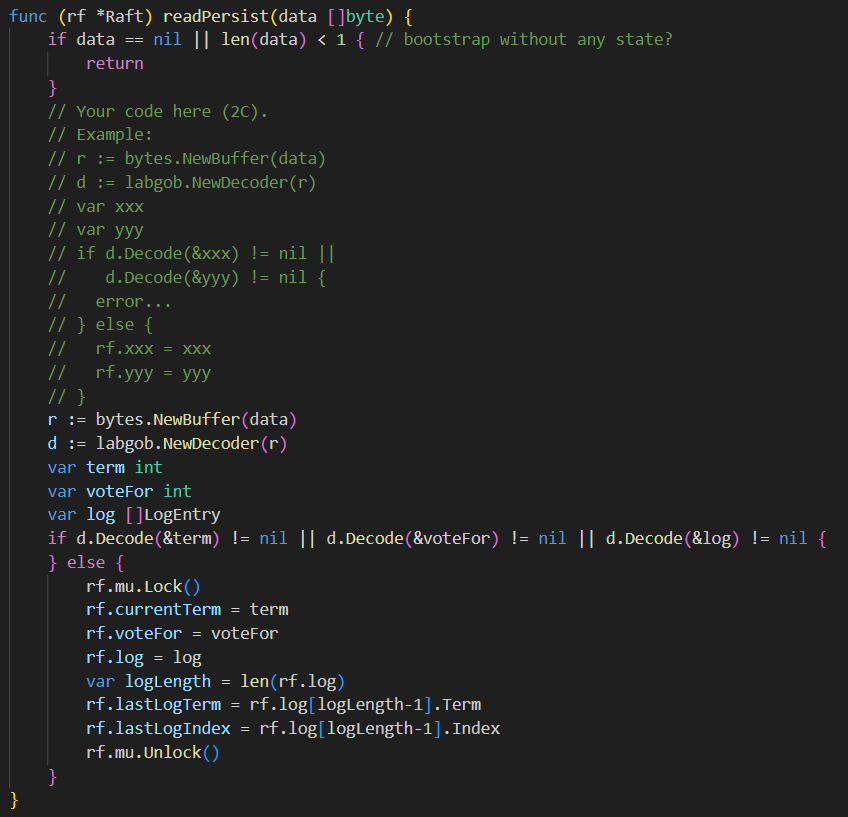
\includegraphics[width=0.8\textwidth]{./2C/readPersist.png}
			\caption{readPersist函数}
		\end{figure}
	\end{itemize}
	\subsection{测试结果}
	\begin{figure}[H]
		\centering
		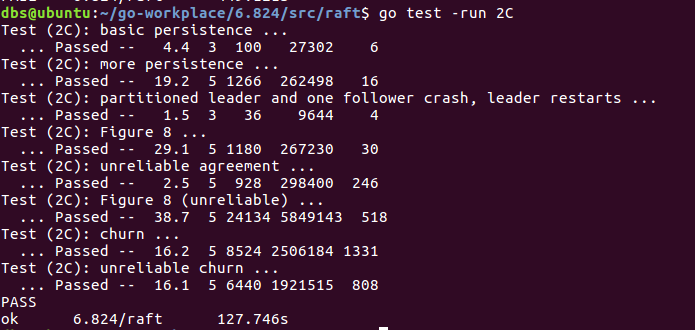
\includegraphics[width=0.8\textwidth]{./2C/2C result.png}
		\caption{2C运行结果}
	\end{figure}
	\begin{figure}[H]
		\centering
		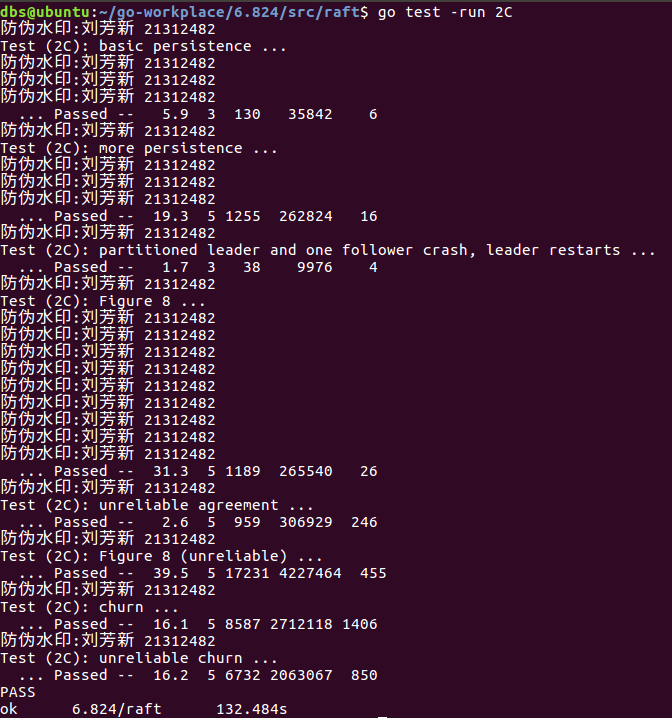
\includegraphics[width=0.75\textwidth]{./2C/2C result1.png}
		\caption{2C运行水印}
	\end{figure}
	\subsection{个人总结}
	Lab 2C目前似乎是对调试能力最大的考验,因为实验中的网络测试环境异常不稳定,极大地考验了程序在网络容错性方面的表现。在处理大量高延迟的网络包、频繁出现网络分区和节点崩溃等问题时,需要在代码中具备较强的容错性。
	
	因此,这个实验的主要工作集中在调试,寻找之前代码中可能存在的漏洞。与此同时,新添加的功能代码量相对较少。主要需要改进的部分似乎在于Log同步阶段,需要我们迅速准确定位leader和follower之间日志一致的位置。
	
	这一过程对调试技能提出了很高的要求,尤其需要高效地解决由于网络不稳定性引起的问题。在这种情况下,细致入微的调试和日志记录将变得尤为重要,以便更有效地定位和解决网络分区和崩溃相关的问题。
	
	\section{心得体会}
	实现Raft协议的过程无疑是对编程能力的一次重大考验。在这个过程中,我查找了大量的资料,经历了多次的尝试和重构。
	
	在这次作业中,由于程序的运行环境是终端而非依赖于IDE调试功能,对于习惯了IDE调试的我感到非常不习惯。在调试的过程中,莫名其妙的bug似乎总是不期而至,为了解决问题,我选择使用插桩法,在每个功能内添加大量的Printf语句以监测程序的运行过程。
	
	面对死锁问题,这似乎成为最大的困难,因为它会使程序在运行时卡住,而又不报错,从而浪费大量的时间。因此,采用Printf语句记录每个步骤的日志成为一种非常有效且必要的手段,帮助我更好地理解程序的运行过程,迅速定位问题并进行解决。
	
	这种经验也反映了在复杂系统设计中,除了理论知识外,调试和日志记录的实际操作也是非常关键的一环。通过这个过程,我不仅仅提升了对Raft协议的理解,还培养了在复杂项目中解决问题的能力。
	
	\section{参考资料}
	\begin{itemize}
		\item MIT 6.824 学习(二)【Raft】 : https://blog.csdn.net/weixin\_48922154/article/details/123956614
		\item MIT 6.824 Lab2 翻译 (已完成)(Raft Base on Golang) : https://zhuanlan.zhihu.com/p/248686289
		\item Lecture 06 - Raft1 : https://mit-public-courses-cn-translatio.gitbook.io/mit6-824/lecture-06-raft1 
		\item 分布式一致性算法:Raft 算法(论文翻译) : https://www.cnblogs.com/linbingdong/p/6442673.html
	\end{itemize}
	
	%	\begin{thebibliography}{100}
		%		\bibitem{ref1}Wang J, Wu R, Chen G, et al. RISC-V Toolchain and Agile Development based Open-source Neuromorphic Processor[J]. arXiv preprint arXiv:2210.00562, 2022.
		%		\bibitem{ref2}罗伯特, 霍夫. 神经形态芯片[J]. 科技创业, 2014 (5): 50-53.
		%		\bibitem{ref3}Miyashita D, Kousai S, Suzuki T, et al. A neuromorphic chip optimized for deep learning and CMOS technology with time-domain analog and digital mixed-signal processing[J]. IEEE Journal of Solid-State Circuits, 2017, 52(10): 2679-2689.
		%		\bibitem{ref4}Vrij A, Fisher R, Mann S, et al. Detecting deception by manipulating cognitive load[J]. Trends in cognitive sciences, 2006, 10(4): 141-142.
		%		\bibitem{ref5}许畅, 高金虎. 认知干预: 战略欺骗的新视角[J]. 情报杂志, 2019, 38(7): 23-27.
		%		\bibitem{ref6}Caccavale R, Finzi A. A robotic cognitive control framework for collaborative task execution and learning[J]. Topics in Cognitive Science, 2022, 14(2): 327-343.
		%	\end{thebibliography}
\end{document}
